\documentclass[11pt]{article}
%\usepackage[T1]{fontenc}
%\usepackage[latin9]{inputenc}
\usepackage[margin=1in]{geometry}
\usepackage{csquotes}
\usepackage{xcolor}

% To compile in Times New Roman, use the following two lines.
% You'll need to compile with xelatex or lualatex.
% If you don't have these compilers, you can outcomment these two lines,
% but it won't be in Times New Roman.
% \usepackage{fontspec}
% \setmainfont{Times New Roman}

\usepackage{sectsty} % to get the section headings to be smaller
\usepackage{natbib}
\usepackage{bbm}
\usepackage{bm}
\usepackage{amsmath,amssymb,amsthm,mathtools}
\usepackage{caption}
\usepackage{subcaption}
\usepackage{algorithmic}
%\usepackage{authblk} % if you are using texlive on macports, install texlive-latex-extra to get this

% Uses the sectsty package to make section headings smaller.
\sectionfont{\fontsize{12}{15}\selectfont}
\subsectionfont{\fontsize{12}{15}\selectfont}

\newcommand{\Prob}{\mathbb{P}}
\newcommand{\E}{\mathbb{E}}
\newcommand{\EI}{\mathrm{EI}}
\newcommand{\Dir}{\mathrm{Dirichlet}}
\newcommand{\PI}{\text{PI}}
\newcommand{\mb}{\mathbf}
\theoremstyle{remark}
\newtheorem{Algorithm}{Algorithm}
\newtheorem{theorem}{Theorem}
\newtheorem{lemma}{Lemma}
\newtheorem{proposition}{Proposition}
\newtheorem*{remark*}{Remark}

\newcommand{\pfcomment}[1]{{\color{blue} PF: #1}}
\newcommand{\jwcomment}[1]{{\color{red} JW: #1}}

\begin{document}

\title{Supporting Information for \enquote{
 Optimal Learning for Discovering and Optimizing Enzymatic Peptide Substrates 
}}

\maketitle
\tableofcontents
\newpage
\part*{SI Text}
  \section{Peptide Optimization with Optimal Learning}

\subsection{Problem Formulation}
We first introduce mathematical notation that allows precise discussion of the POOL methodology. Let $E$ be the set of peptides over which we would like to search.
In our application, the set $E$ will be the set of peptides of length less than 38 amino acids.
For any peptide $e \in E$, let $y(e) \in \{0, 1\}$ be a binary label indicating whether
the peptide $e$ is a ``hit''.  We suppose that this label can be observed directly through experiment, but is otherwise unknown {\it a priori}.
In our application, we consider two definitions of $y(e)$, depending on whether we are searching for peptides with Sfp-type or AcpS-type activity:
\begin{itemize}
\item When searching for peptides with Sfp-type activity, we let $y(e)$ be $1$ if the peptide is a substrate for both Sfp and AcpH, but is not a substrate for AcpS.  We call this an \enquote{Sfp-type hit}.
\item When searching for peptides with AcpS-type activity, we let $y(e)$ be $1$ if the peptide is a substrate for both AcpS and AcpH, but is not a substrate for Sfp.  We call this an \enquote{AcpS-type hit}.
\end{itemize}

POOL searches for peptides that are hits, and for which another given fitness function $f(e)$ is large.   We assume that this fitness function can be observed directly without requiring a physical experiment. In our application, the fitness is negative one times the length of the peptide.  The negative one is present because we will want fitness to be large, but we want the length to be small.

Our goal, in terms of the notation we have defined, is to find a peptide $e\in E$ for which $y(e)=1$ and for which $f(e)$ is as large as possible.  We can write this problem as,
\begin{equation}
  \underset{e \in E, y(e) = 1}{\arg\max} \, f(e).
  \label{eq:general problem}
\end{equation}

However, we typically cannot solve this problem directly because $y(e)$ has only been observed for those peptides on which we have performed an experiment, which is typically only a small fraction of the peptides in our search space $E$, and the additional experimental effort required to observe $y(e)$ for all peptides in $E$ is simply beyond the realm of feasibility.  
For example, in our application, $E$ contains more than $2 \times 10^{49}$ peptides. Our current experimental approach allows testing roughly $600$ peptides for one round, and we can only perform $4$ rounds of experiments in total. Therefore, we only have the budget to test a tiny fraction of $E$ in searching for peptide hits.

POOL is designed for these situations in which the number of peptides we can evaluate is substantially smaller than the search space.  
It assumes that we have available the values of $y(e)$ for a small number of previously evaluated peptides (we refer to this as ``training data''), and that we can also evaluate $y(e)$ for a set of new peptides chosen by POOL.  POOL supposes that peptides are evaluated in batches, and we let $M$ denote the number of peptides in a batch.  POOL may be applied once, to recommend a single batch of peptides to test, or it may be applied repeatedly, each time adding the results from previously tested batches to the training data.

%In our application, our training data initially contained data allowing partial evaluation of $y(e)$, for 14 proteins (length longer than 38) from the literature \jwcomment{Add cites to papers for the initial data}, as well as one length-11 peptide obtained using phage display by~\cite{yin2005genetically}.
%We did 5 rounds using a batch size $k$ that varied somewhat from batch to batch, but remained approximately equal to 500.

POOL uses such limited evaluation budgets to best support solving \eqref{eq:general problem}, in the specific sense of maximizing the probability of finding a peptide hit whose quality is better than some target quality $b$.
It consists of two steps: first, a prediction step, in which a machine learning method (Bayesian Na{\"i}ve Bayes classifier, customized for peptide activity) provides a joint probability distribution over peptide activity; second, a probability-of-improvement step, in which we use value-of-information analysis to define the quality of a set of peptides to test, and then use an approximation algorithm to find a set of peptides to test that provides a large probability-of-improvement.

We discuss POOL in more detail in the following sections: Sect.~\ref{sec:model} describes the Bayesian Na{\"i}ve Bayes classifier that predicts the peptide activity;
Sect.~\ref{sec:voi} provides the value-of-information analysis and the approximation algorithm in POOL;
Sect.~\ref{sec:contrast with predict-then-optimize} discusses why POOL performs better than the ``predict-then-optimize'' approach.

\subsection{Prediction Model: Bayesian Na{\"i}ve Bayes Classifier}  \label{sec:model}

In the prediction step of POOL, we build a Bayesian Na{\"i}ve Bayes classifier as the underlying machine learning model to predict the joint probability distribution over peptide activity.

Na{\"i}ve Bayes classifiers~\cite{lewis1994sequential, mccallum1998comparison} are popular and extensively studied in text classification problems because of their fast computation and simple implementation.
Peptides are sequences of amino acids, which have big influence on peptide activity, and this is very similar to text classification, where words within text influence on which class the text belongs to, therefore, a Na{\"i}ve Bayes classifier is suitable for peptide activity prediction. 
In addition, we usually do not afford to have a training dataset with thousands of data points in peptide activity, the independence assumption across features in Na{\"i}ve Bayes allows it to achieve good prediction performance even when the data size is small, which is desirable in the problems that we are dealing with.

To describe the model, let $X=(X_1,\ldots,X_L)$ be a feature vector and $Y$ be its label. Using Bayes' Rule, we have:

\begin{equation*}
\Prob(Y=y|X=x)=\frac{\Prob(X=x|Y=y)\Prob(Y=y)}{\Prob(X=x)}=\frac{\Prob(X=x|Y=y)\Prob(Y=y)}{\sum_{y'}\Prob(X=x|Y=y')\Prob(Y=y')}.
\end{equation*}

The Na{\"i}ve Bayes classifier assumes that the presence or absence of a particular feature is unrelated to the presence or absence of any other feature, given the class variable, i.e.

\begin{equation*}
\Prob(Y=y|X=x) = \frac{\prod_{j=1}^L\Prob(X_j=x_j|Y=y)\Prob(Y=y)}{\sum_{y'}\prod_{j=1}^L\Prob(X_j=x_j|Y=y)\Prob(Y=y)}.
\end{equation*}

In the context of our application, $Y$ is a random variable that is either ``1'' or ``0'', depicts whether a peptide is a ``hit'' or ``miss''; $X$ is feature vector
that encodes any peptide of interest, which is designed in the following: since a peptide is a sequence of amino acids, we use $A_j \in \{1, \ldots, 20\}$ to indicate 
the type of amino acid in $j$th position of the sequence, where $j=1,\ldots,L$; we further partition the 20 different types of amino acids into $K$ groups ($K \leq 20$)
according to their biochemical similarities, then $j$th feature is simply indicating which group the amino acid in the $j$th position of the sequence belongs to, denoted
as $x_j$.

We let $\theta_{y,j}(k)=\Prob(X_i=k|Y(X)=y)$, where $j=1,\ldots,L$, $k=1,\ldots,K$ and $y\in\{0,1\}$. Then given a prior distribution $\Prob(Y(x)=y)$, $y\in\{0,1\}$, the
Bayesian inference for any peptide $x$ is
%Let $\theta$ be the full set of parameters $\theta_{y,j}(k)$, for $j=1,\ldots,L$, $k=1,\ldots,K$ and $y\in\{0,1\}$. Then, given an unlabeled peptide, we can calculate its probability of being a substrate as:
%
\begin{equation} \label{eq:peptide model}
  \Prob\left(Y(x) = 1 | \boldsymbol{\theta}_0, \boldsymbol{\theta}_1, x \right) =
  \frac{\Prob(Y(x)=1) \prod_{j} \theta_{1,j}(x_j)}{
  \left[ \Prob(Y(x)=1) \prod_{j} \theta_{1,j}(x_j)\right] +
  \left[ \Prob(Y(x)=0) \prod_{j} \theta_{0,j}(x_j)\right]},
\end{equation}
where $\boldsymbol{\theta}_0$ and $\boldsymbol{\theta}_1$ are the matrix representations of $\theta_{0,j}(k)$ and $\theta_{1,j}(k)$. 

We train the model parameters $\theta_{y,j}(k)$ using Bayesian inference. We assume the prior distribution over $\theta_{y,j}(\cdot)$ is 
$\Dir(\alpha_{y,j}(1),\ldots,\alpha_{y,j}(K))$, and we 
can encode prior knowledge from domain experts into the choices of the prior parameters $\alpha_{y,j}(k)$. In this biochemical application, the enzymes can only
attach/detach ``label'' to/from a special position in the peptide, and we know that those positions further away from this special position will have less
influence on whether the peptide is a hit or not. To encode this information into the prior, we increase the value of $\alpha_{y,j}(k)$ and make it uniform over
$k$ as $j$ moves further away from the known position, and this encodes the belief that the positions far away from the special position is less sensitive about
which amino acid to appear over that position.
%
From Bayesian statistics, we know that the posterior is $\Dir( \alpha_{y,j}(1) + N_{y,j}(1), \ldots, \alpha_{y,j}(K) + N_{y,j}(K))$, where $N_{y,j}(k)$ is the number
of the peptides in the training set with $Y(x)=y$, and $x_j=k$.
%
Now we have constructed the model for predicting peptide activity and the method of updating model parameters given data.

\subsection{The Contingency Plan: Value-of-information Analysis}  \label{sec:voi}
We have described how POOL method builds a contingency plan in finding the peptides that are likely to be hits in the main article. In this section, we show how
this approach is derived mathematically. We provide an outline for this section here: 
Sect.~\ref{sec:prob improvement} discusses value-of-information analysis and gives the high-level strategy of constructing the set of peptides to test next;
Sect.~\ref{sec:greedy algorithm} provides an approximation algorithm to solve the otherwise difficult-to-solve objective given in~\ref{sec:greedy algorithm}, and
proves that this approximation algorithm has a performance guarantee;
Sect.~\ref{sec:reduced form} further simplifies the approximation algorithm, and derives the main procedures of POOL;
Sect.~\ref{sec:MINLP approach} and~\ref{sec:MAP approach} provide two implementations of the approximation algorithm.

\subsubsection{Probability-of-improvement} \label{sec:prob improvement} 
Given the prediction model, the Bayesian optimization approach uses decision theory to suggest which points in the function's domain would be the most valuable
to evaluate next, known as the value of information analysis. In our application, a point in the function's domain corresponds to a peptide, and therefore, we
use value-of-information analysis to decide the set of peptides to test next in finding peptide hits. Specifically, we use an information criterion, which is a
function, to quantify the information gain if we were to test a given set of peptides, and then our goal is to find the set of peptides that maximizes this
information gain.

Probability-of-improvement is one such criterion, initially proposed by~\cite{kushner1964new}. In this context, the probability-of-improvement quantifies the 
probability that a set of peptides $S$, if tested, will reveal a hit whose fitness $f(e)$ improves on some benchmark value $b$, 
which is typically the best $f(e)$ of hits observed in the past. We define this probability-of-improvement, $\PI(S)$, to be
\begin{equation}
  \PI(S) = \Prob \left( \max_{e \in S, y(e)=1} f(e) > b \right).
  \label{}
\end{equation}
To ensure the event that none of the peptides we test is hit does not contribute to probability-of-improvement, we define $\max$ over an empty set is $-\infty$. We find $S$ by solving
\begin{equation}
  \underset{S \subseteq E, |S| \leq M}{\arg\max} \PI(S),
  \label{eq:opt PI}
\end{equation}
where $M$ is the number of peptides that can be tested simultaneously in a single round of experiment. 

After we find the set $S$ and test this set of peptides, we obtain the labels for these peptides that whether they are hits or not. We update our prediction model 
in Sect.~\ref{sec:model} with the new data, and solve~\eqref{eq:opt PI} again to obtain a new set of peptides to test for the next round of experiment.
We repeat this process until we find enough hits or resource is exhausted. We have just described the high-level approach of POOL, however, solving~\eqref{eq:opt PI}
when $E$ and $M$ are large is very difficult. In this application, the size of $E$ is in the order of $10^{49}$ and $M \approx 600$, and therefore brute-force approach
is not feasible. The rest of the section is dedicated to proposing an approximation algorithm to solve~\eqref{eq:opt PI}, and proving its performance guarantee. 

\subsubsection{Greedy Algorithm and Its Performance Guarantee} \label{sec:greedy algorithm}
Directly solving~\eqref{eq:opt PI} is computationally challenging, because the size of the search space $|E|^M$, which grows exponentially in $M$. 
Therefore we propose to use greedy algorithm to solve it approximately, that is, we begin with $S = \emptyset$, and add one peptide at a time to $S$ by solving
\begin{equation}
  \underset{e \in E \backslash S}{\mathrm{arg}\max} \,\PI (S \cup \{e\}),
  \label{eq:greedy}
\end{equation}
until $|S| = M$. This algorithm is much less computational challenge because we reduced the size of the search space from $|E|^M$ down to $|E|$. We also show in
the following theorem that the this algorithm has a performance guarantee compared to the optimal solution.

\begin{theorem} \label{thm:greedy}
  The greedy algorithm always produces a solution whose probability-of-improvement is at 
  least $1-[(k-1)/k]^k \geq 1 - 1 / e$ times the optimal solution of~\eqref{eq:opt PI}.
\end{theorem}
To prove the theorem, we use the following two lemmas:
\begin{lemma}  \label{lemma:1}
  If $F(S)$ is submodular, non-decreasing and $F(\emptyset)=0$, the greedy heuristic always 
  produces a solution whose value is at least $1-[(k-1)/k]^k$ times the optimal value, where 
  $|S| \leq k$. This bound can be achieved for each $k$ and has a limiting value of $1-1/e$, 
  where $e$ is the base of the natural logarithm.
\end{lemma}
Lemma~\ref{lemma:1} is a result from the analysis of greedy heuristics in combinatorial optimization by 
Nemhauser~\cite{nemhauser1978analysis}, which provides lower bound on the greedy algorithm given that the objective function 
satisfies certain conditions. To show that this lemma applies to Theorem~\ref{thm:greedy}, we need to show our objective function,
which is probability-of-improvement, satisfies the conditions given in Lemma~\ref{lemma:1}. Lemma~\ref{lemma:2} to be stated below 
shows that probability-of-improvement indeed satisfies these conditions, and therefore concludes the theorem.

\begin{lemma} \label{lemma:2}
  Probability-of-improvement $\PI(S)$ is submodular, non-decreasing and $\PI(\emptyset)=0$.
\end{lemma}
\begin{proof}
Let $f^*(S) = \max_{e \in S, y(e)=1} f(e)$. First we show $\PI(\emptyset) = 0$.
\begin{equation*}
  \PI(\emptyset) = \Prob(f^*(\emptyset) > b) = \Prob(-\infty > b)=0.
\end{equation*}

To show $\PI(S)$ is non-decreasing, let $A \subseteq B \subseteq E$ where $E$ is a finite set, then
\begin{equation*}
\begin{split}
\PI(B) &= \Prob(f^*(B) > b) \\
       &= \Prob(f^*(B) > b \mid f^*(A) \leq b) \Prob(f^*(A) \leq b) + \Prob(f^*(B) > b \mid f^*(A) > b) \Prob(f^*(A) > b) \\
       &= \Prob(f^*(B) > b \mid f^*(A) \leq b) \Prob(f^*(A) \leq b) + \Prob(f^*(A) > b) \\
       &\geq \Prob(f^*(A) > b) \\
       &= \PI(A).
\end{split}
\end{equation*}

Lastly, we want to show $\PI(S)$ is submodular. For $e \in E\backslash B$,
\begin{equation*}
  \begin{split}
    &\PI(A \cup \{e\}) - \PI(A) \\
    &= \Prob(f^*(A \cup \{e\}) > b) - \Prob(f^*(A) > b) \\
    &= \Prob(f^*(A \cup \{e\}) > b \mid f^*(A) > b) \Prob(f^*(A) > b) \\
    &\quad + \Prob(f^*(A \cup \{e\}) > b \mid f^*(A) \leq b)
    \Prob(f^*(A) \leq b) - \Prob(f^*(A) > b) \\
    &= \Prob(f^*(A \cup \{e\}) > b \mid f^*(A)\leq b) \Prob(f^*(A)\leq b) \\
    &= \Prob(f(e) > b, y(e) = 1 \mid f^*(A) \leq b) \Prob(f^*(A) \leq b) \\
    &= \Prob(f(e) > b, y(e) = 1, f^*(A) \leq b).
  \end{split}
\end{equation*}
Using similar argument,
\begin{equation*}
\begin{split}
&\PI(B \cup \{e\}) - \PI(B) \\
&= \Prob(f(e) > b, y(e)=1,f^*(B)\leq b) \\
&= \Prob(f(e) > b, y(e)=1,f^*(A)\leq b, f^*(B\backslash A) \leq b ).
\end{split}
\end{equation*}
Therefore, $\PI(A \cup \{e\}) - \PI(A) \geq \PI(B \cup \{e\}) - \PI(B)$, thus $\PI(S)$ is submodular. \qedhere
\end{proof}

\begin{remark*}
  The theoretical result we have obtained so far does not use any information about the prediction model we used in Sect.~\ref{sec:model}, 
  which means Theorem~\ref{thm:greedy} is a general result for our greedy algorithm, independent from the choice of prediction model.
  Therefore, even one uses a different prediction model than in Sect.~\ref{sec:model} in this greedy algorithm, the same result applies.
\end{remark*}

\subsubsection{A Simplified Form of the Greedy Algorithm} \label{sec:reduced form}
\eqref{eq:greedy} is still hard to solve, at least in a naive way, where we simply enumerate all peptides $e \in E \backslash S$ 
and evaluate $\PI (S \cup \{e\})$ for each of them, and then select the peptide for which the $\PI$ is the largest. It is hard because
first, the peptide space $E$ in our application is too large to enumerate over all of the peptides, and second, computing $\PI(\cdot)$
for each enumeration is expensive because its computational cost increases linearly in the size of $S$. We can transform~\eqref{eq:greedy}
into a simplified form so that 1. we solve the same problem without having to evaluate $\PI(\cdot)$, and 2. it paves the way for using
more efficient methods to solve the problem as discussed in Sect.~\ref{sec:MINLP approach} and~\ref{sec:MAP approach}. We show the 
simplified form in the following proposition:

\begin{proposition} \label{prop:reduced form}
  The solution to \eqref{eq:greedy} is equivalent to
  \begin{equation}
    \underset{e \in E \backslash S, f(e) > b}{\mathrm{arg}\max} \, \Prob (y(e)=1 \mid y(e') = 0, \forall e' \in S).
    \label{eq:reduced form}
  \end{equation}
\end{proposition}
\begin{proof}
  The objective in~\eqref{eq:greedy} can be written as
  \begin{equation*}
    \begin{split}
      &\PI(S \cup \{e\}) \\
      &= \Prob(f^*(S\cup \{e\}) > b),\\
      &= \Prob(f^*(S) > b) + \Prob(f^*(S)\leq b) \Prob(f(e) > b, y(e) = 1 \mid f^*(S)\leq b).
    \end{split}
  \end{equation*}
  Because $S$ is a constant in~\eqref{eq:greedy}, the following equality holds:
  \begin{equation} \label{eq:PI1} 
    \underset{e \in E \backslash S}{\arg\max} \, \PI(S \cup \{e\}) = \underset{e \in E \backslash S}{\arg\max} \, \Prob(f(e) > b, y(e)=1 \mid f^*(S)\leq b).
  \end{equation}
  When $f(e) \leq b$, the objective in~\eqref{eq:PI1}, $\Prob(f(e) > b, y(e) = 1 \mid f^*(S)\leq b)$ evaluates to zero; when $f(e) > b$, this objective is 
  always greater or equal to zero because it is a probability function. Therefore, \eqref{eq:PI1} is equivalent to
  \begin{equation*}
    \underset{e \in E \backslash S, f(e) > b}{\arg\max} \, \Prob (y(e) = 1 \mid y(e') = 0, \forall e' \in S). 
  \end{equation*}
\end{proof}

The formulation in Proposition~\ref{prop:reduced form} conveys exactly the same message as the verbal description of the POOL method in the main text: we
construct the set $S$ by adding the top-scoring peptide iteratively, i.e., the most probable being a hit, according to the prediction model trained on all previously
observed data plus the peptides that are already in $S$ and assume none of them is a hit. Here we provided the mathematical derivation for the POOL method.

Note that the derivation so far remains independent from the choice of prediction model, and therefore, the POOL method and its performance guarantee
apply to any prediction model as long as the objective in~\eqref{eq:reduced form} can be evaluated.

\subsubsection{POOL-MINLP: Solve the Greedy Step using MINLP} \label{sec:MINLP approach}
Solving \eqref{eq:reduced form} by simply brute-force search still remains infeasible when the search space $E$ is large. In our application,
$E$ contains more than $2 \times 10^{49}$ peptides, and if evaluating for one peptide takes $\sim 10^{-3}$ seconds, it will
require more than $2 \times 10^{46}$ seconds to complete all evaluations. 

To solve this problem more efficiently, we formulate~\eqref{eq:reduced form} as an instance of Mixed-Integer Nonlinear Program (MINLP), 
and then we can use any MINLP solver to solve \eqref{eq:reduced form} efficiently. 
Let $\theta^{y', j}_{x_j} = \Prob \left( x_j \mid y(e) = y' \right)$, from~\eqref{eq:peptide model} we have
\begin{equation}
\begin{split}
  \Prob \left(y(e \right) = 1 \mid \bm{x}) &= \frac{\prod_{j=1}^J \theta^{1, j}_{x_j} \Prob\left( y(e)=1 \right)}{\prod_{j=1}^J \theta^{1, j}_{x_j} \Prob\left( y(e)=1 \right) + \prod_{j=1}^J \theta^{0, j}_{x_j} \Prob\left( y(e)=0 \right)}, \\
  &= \frac{\prod_{j = 1}^J \eta^j_{x_j}}{\prod_{j=1}^J \eta^j_{x_j} + \frac{\Prob \left(y(e) = 0 \right)}{\Prob \left( y(e) = 1 \right)}},
  \label{eq:MINLP_2}
\end{split}
\end{equation}
where $\eta^j_{x_j} = \frac{\theta^{1,j}_{x_j}}{\theta^{0,j}_{x_j}}$ for $\forall j \in \{1,\ldots,J\}$. Since $\theta^{y'}_{x_j}$s are unknown model parameters,
we use Bayesian inference as described in Sect.~\ref{sec:model} to estimate the posterior probability over them. We then compute expectation of~\eqref{eq:MINLP_2}
using the posterior probability distribution, written as
\begin{equation}
  \hat{\Prob} \left(y(e \right) = 1 \mid \bm{x}) = \E \left[ \frac{\prod_{j = 1}^J \eta^j_{x_j}}{\prod_{j=1}^J \eta^j_{x_j} + \frac{\Prob \left(y(e) = 0 \right)}{\Prob \left( y(e) = 1 \right)}} \right].
  \label{eq:MINLP_3}
\end{equation}

To compute~\eqref{eq:MINLP_3}, we use sample average approximation \cite{kleywegt2002sample}, in which we sample 
$R$ i.i.d. samples from the posterior distributions of $\bm{\theta}^{1, j}$ and $\bm{\theta}^{0, j}$ 
(they are Dirichlet distributions with parameters given in Sect.~\ref{sec:model}). 
We then approximate \eqref{eq:MINLP_3} by 
\begin{equation}
\hat{\Prob} \left(y(e \right) = 1 \mid \bm{x}) = \frac{1}{R} \sum_{r = 1}^R \frac{\prod_{j=1}^J \eta^{j, r}_{x_j}}{\prod_{j=1}^J \eta^{j, r}_{x_j} + \frac{\Prob \left(y(e) = 0 \right)}{\Prob \left( y(e) = 1 \right)}}.
\label{eq:MINLP_4}
\end{equation}

Now we can replace the objective in~\eqref{eq:reduced form} by~\eqref{eq:MINLP_4}, and formulate~\eqref{eq:reduced form} into a MINLP:
%Now we can apply the approximate expression to \eqref{eq:reduced form}, by sampling from posterior distribution of 
%$\bm{\theta}^{1, j}$ and $\bm{\theta}^{0, j}$ given all training data and $\{y(e') = 0, \forall e' \in S\}$. We write 
%\eqref{eq:reduced form} as a Mixed-Integer Nonlinear Program,
\begin{equation}
  \begin{split}
    \max \quad & \sum_{r = 1}^R \frac{\prod_{j=1}^J \sum_{k=1}^{K_j} z^j_k \eta^{j, r}_k}
    {\prod_{j=1}^J \sum_{k=1}^{K_j} z^j_k \eta^{j, r}_k + \frac{\Prob \left(y(e) = 0 \right)}{\Prob \left( y(e) = 1 \right)}}, \\
    \text{s.t} \quad &z^j_k \in \{0,1\}, \\
    &\sum_{k=1}^{K_j} z^j_k = 1, \,\, \forall j \in \{1, \ldots, J\},
  \end{split}
  \label{eq:MINLP_5}
\end{equation}
where $z^j_k$ is indicative variables that equal to 1 if $x_j = k$ and 0 otherwise, and $\eta_k^{j,r}, r=1,\ldots,R$ are computed using i.i.d. samples from
the posterior distribution of $\bm{\theta}^{1, j}$ and $\bm{\theta}^{0, j}$ given the previously observed data plus the additional ``data'' $\{y(e')=0, \forall e' \in S\}$.
Suppose the solution to~\eqref{eq:MINLP_5} is $\bm{z}^*$, we can translate it to the feature representation $\bm{x}^*$ by letting $x^{*j} = \sum_k k \cdot z^{*j}_k$.

%There is an additional constraint in \eqref{eq:reduced form}, $f(e) > b$, that we did not include in \eqref{eq:MINLP_4}. This
%constraint depends on the definition of $f(e)$, and if $f(e) > b$ can be represented by a set of linear inequalities
%of $\bm{x}$, we can simply add those constraints to our MINLP in \eqref{eq:MINLP_4}. In our application, $f(e)$ is negative the length
%of a peptide, thus the additional constraint to \eqref{eq:MINLP_4} is simply to restrict length of peptide to less than $-b$. 
We summarize the algorithm below, in which the output $S$ is the set of peptides to test next. 
\begin{Algorithm}(Greedy Algorithm for POOL-MINLP) \label{algo1}
\begin{algorithmic}[1]
  \REQUIRE Inputs $M, J, R, K_j, j = 1, \ldots, J$, training dataset $\mathcal{D} = 
  \{(\bm{x}^1, y^1), \ldots, (\bm{x}^N, y^N)\}$ and parameters for the prior 
  distributions $\bm{\alpha}^{y, j}$.
  \STATE $S \leftarrow \emptyset $
  \STATE Calculate posterior distribution of $\bm{\theta}^{1, j} \sim 
  \text{Dirichlet} (\bm{\theta}^{1, j} \mid \{\bm{x}: \bm{x} \in \mathcal{D}, 
  y(\bm{x}) = 1\})$ for $j = 1, \ldots, J$.
  \FOR{$m=1$ to $M$} 
    \STATE Calculate posterior distribution of $\bm{\theta}^{0, j} \sim 
    \text{Dirichlet} (\bm{\theta}^{0, j} \mid \{\bm{x}: \bm{x} \in \mathcal{D}, 
    y(\bm{x}) = 1\} \cup S)$ for $j = 1, \ldots, J$.
    \FOR{$r=1$ to $R$}
      \FOR{$j=1$ to $J$}
          \STATE Sample $\bm{\theta}^{1, j}$ from $\text{Dirichlet} (\bm{\theta}^{1, j} 
          \mid \{\bm{x}: \bm{x} \in \mathcal{D}, y(\bm{x}) = 1\})$ and $\bm{\theta}^{0, j}$
          from $\text{Dirichlet} (\bm{\theta}^{0, j} \mid \{\bm{x}: \bm{x} \in \mathcal{D}, 
          y(\bm{x}) = 1\} \cup S)$.
          \STATE Calculate $\bm{\eta}^{j, r}_i = \frac{\theta^{1, j}_i}{\theta^{0, j}_i}, \forall i \in K_j$.
      \ENDFOR
    \ENDFOR
    \STATE Solve the MINLP in~\eqref{eq:MINLP_5} to find $\bm{z}^*$ and the corresponding peptide $e$.
    \STATE $S \leftarrow (S, e)$.
  \ENDFOR
\end{algorithmic}
\end{Algorithm}

\subsubsection{POOL-MAP: Solve the Greedy Step using MAP Estimation} \label{sec:MAP approach}
In our application, due to the large peptide space, the MINLP approach still takes hours to solve~\eqref{eq:reduced form}, and since
$M=600$ in the application, the overall time to complete Algorithm~\ref{algo1} is $600$ times the a few hours for solving~\eqref{eq:reduced form},
which is too long given the time constraint.

To deal with this problem, we propose a simpler approach using Maximum a Posteriori (MAP) estimation~\cite{trove.nla.gov.au/work/9892361}. 
Although this approach less accurate than the MINLP approach, the computation is much cheaper and faster.

We first obtain the posterior distributions of $\bm{\theta}^{1, j}$ and $\bm{\theta}^{0, j}$ for $\forall j \in \{1, \ldots, J\}$, same as before.
We then approximate~\eqref{eq:MINLP_2} using posterior mode $\hat{\theta}^{1,j}_i$ and $\hat{\theta}^{0,j}_i$, written as 
\begin{equation*}
  \hat{\Prob} \left(y(e \right) = 1 \mid \bm{x}) = \frac{\prod_{j=1}^J \hat{\theta}^{1, j}_{x_j} \Prob\left( y(e)=1 \right)}{\prod_{j=1}^J \hat{\theta}^{1, j}_{x_j} \Prob\left( y(e)=1 \right) + \prod_{j=1}^J \hat{\theta}^{0, j}_{x_j} \Prob\left( y(e)=0 \right)}.
\end{equation*}
This estimation is known as Maximum a posteriori estimation. Now we can write~\eqref{eq:reduced form} as 
\begin{equation}
  \underset{\bm{x}}{\arg\max} \frac{\prod_{j=1}^J \hat{\eta}^j_{x_j}}{\prod_{j=1}^J \hat{\eta}^j_{x_j} + \frac{\Prob \left(y(e) = 0 \right)}{\Prob \left( y(e) = 1 \right)}},
  \label{eq:MINLP_6}
\end{equation}
where $\hat{\eta}^j_{x_j} = \frac{\hat{\theta}^{1,j}_{x_j}}{\hat{\theta}^{0,j}_{x_j}}$. Since $\hat{\eta}^j_i \geq 0$, the objective 
in~\eqref{eq:MINLP_6} is monotone increasing with $\hat{\eta}^j_{x_j}, \forall j$. Therefore we can solve~\eqref{eq:MINLP_6} by
maximizing $\prod_{j=1}^J \hat{\eta}^j_{x_j}$ over $\bm{x}$. Since $\hat{\eta}^j_{x_j}$ are independent across $j$ by the assumption of the 
Na{\"i}ve Bayes model, we can decompose the objective across $j$ and maximize $\hat{\eta}^j_{x_j}$ by setting 
$x_j = \underset{i}{\arg\max} \, \hat{\eta}^j_i, \forall j$. The property of decomposition across $j$ in this formulation makes the
optimization problem a lot easier and requires much less computation effort than the POOL-MINLP approach. We summarize the algorithm below:
\begin{Algorithm}(Greedy Algorithm for POOL-MAP) \label{algo2}
\begin{algorithmic}[1]
  \REQUIRE Inputs $M, J, K_j, j = 1, \ldots, J$, dataset $\mathcal{D} = 
  \{(\bm{x}^1, y^1), \ldots, (\bm{x}^N, y^N)\}$ and parameters for the prior 
  distributions $\bm{\alpha}^{y, j}$.
  \STATE $S \leftarrow \emptyset $
  \STATE Calculate posterior distribution of $\bm{\theta}^{1, j} \sim 
  \text{Dirichlet} (\bm{\theta}^{1, j} \mid \{\bm{x}: \bm{x} \in \mathcal{D}, 
  y(\bm{x}) = 1\})$.
  \FOR{$m=1$ to $M$} 
    \STATE Calculate posterior distribution of $\bm{\theta}^{0, j} \sim 
    \text{Dirichlet} (\bm{\theta}^{0, j} \mid \{\bm{x}: \bm{x} \in \mathcal{D}, 
    y(\bm{x}) = 1\} \cup S)$.
    \STATE Calculate posterior mode $\hat{\theta}^{1, j}_i$ and $\hat{\theta}^{0, j}_i$ for $\forall i \in K_j, j = 1, \ldots, J$, and $\hat{\eta}^j_i = \frac{\hat{\theta}^{1, j}_i}{\hat{\theta}^{0, j}_i}$.
    \STATE Construct $\bm{x}$ by setting $x_j = \underset{i}{\arg\max} \, \hat{\eta}^j_i, \forall j$, and find the corresponding peptide $e$.
    \STATE $S \leftarrow (S, e)$.
  \ENDFOR
\end{algorithmic}
\end{Algorithm}

\subsection{How POOL Combats Prediction Errors} \label{sec:contrast with predict-then-optimize}
We have compared POOL with a closely related benchmark method in the main text, the ``predict-then-optimize'' method, which uses the same prediction model
as POOL. Suppose the prediction model is highly accurate, then the ``predict-then-optimize'' method should have a comparable performance v.s. POOL, or even
better. However, in the benchmark experiments we have shown in the main text, POOL has a far superior performance than ``predict-then-optimize''. This is
because our prediction model is not accurate for the prediction, and POOL is better in combating the prediction error while still giving good recommendations.

In this section, we use a simple example to explain how POOL combats the potential prediction errors.
Suppose there are three peptides, $A, B$ and $C$; A and B are very similar to each other, 
and their predicted probability being a hit are both $0.9$, written as $\Prob (A \text{ is a hit}) = \Prob (B \text{ is a hit}) = 0.9$, 
while $C$ is different from $A$ or $B$, and $C$ has a lower predicted probability being a hit, say $\Prob (C \text{ is a hit}) = 0.8$.
We now want to find a hit from these three peptides, and due to budget limit, we could only test two peptides.

The ``predict-then-optimize'' approach will propose to test $A$ and $B$, because they have higher predicted probabilities being a hit. 
However, choosing $A$ and $B$ does not necessarily obtain the highest probability-of-improvement. To demonstration this point, 
we first assume the correlation between $A$ being a hit and $B$ being a hit is $1$, $A$ being a hit and $B$ being a hit 
are both independent from $C$ being a hit, and $f(A), f(B), f(C)$ are all greater than $b$. We compute probability-of-improvement
of choosing $A$ and $B$, that is
\begin{equation*}
\begin{split}
\PI (\{A, B\}) &= \Prob (A \text{ is a hit}, B \text{ is a hit}) + \Prob (A \text{ is a hit}, B \text{ is not a hit}) + \Prob (A \text{ is not a hit}, B \text{ is a hit}), \\
&= 0.9 + 0 + 0, \\
&= 0.9.
\end{split}
\end{equation*}
However, probability-of-improvement of choosing $A$ and $C$ is
\begin{equation*}
\begin{split}
\PI (\{A, C\}) &= \Prob (A \text{ is a hit}, C \text{ is a hit}) + \Prob (A \text{ is a hit}, C \text{ is not a hit}) + \Prob (A \text{ is not a hit}, C \text{ is a hit}), \\
&= 0.9 \times 0.8 + 0.9 \times 0.2 + 0.1 \times 0.8, \\
&= 0.98.
\end{split}
\end{equation*}
Similarly, $\PI(\{B, C\})=0.98$. Therefore, POOL, which recommends peptides that maximize probability-of-improvement, will choose either 
$\{A, C\}$ or $\{B, C\}$. Now suppose $A$ (or $B$) turns out to be a miss after
the experiment, then $B$ (or $A$) is unlikely to be a hit either because $A$ and $B$ are very similar to each other. On the other hand, since $C$ is 
different than $A$ and $B$, there might be a chance that $C$ is a hit even if $A$ or $B$ is not a hit. 
Therefore, choosing diversified and good peptides to test, i.e., choosing $\{A, C\}$ or $\{B, C\}$ in this example, 
is a better strategy than choosing peptides with high predicted value regardless of diversity, i.e., choosing $\{A, B\}$. This diversity
is the key to finding hits when the prediction model is not accurate.

\subsection{Predicting Multiple Activities} \label{sec:extension}
In our application, we are looking for peptides satisfying multiple criteria. Since the experimental setup allows us to observe whether
a peptide satisfies for each individual criterion, instead of simply using hits that satisfy all criteria as our data, we build
seperate models for predicting each individual criterion, that is, we predict $y_i(e)$ for a peptide $e$, where $y_i(e)$ is $1$ if
the peptide satifies $i$th criterion, or zero otherwise. Then $\prod_i y_i(e)$ tells whether the peptide $e$ is a hit that satisfies
all criteria or not. This approach allows us to make full use of all observational data we can obtain, and is also flexible suppose we were to look for a
different combination of criteria.

We then need to rewrite~\eqref{eq:reduced form} as

\begin{equation*}
  \underset{e \in E \backslash S, f(e) > b}{\mathrm{arg}\max} \, \Prob (y_i(e)=1, \forall i \mid \prod_i y_i(e') = 0, \forall e' \in S).
\end{equation*}
This objective is hard to compute because the number of configurations of $y_i(e'), \forall e \in S$ that satisfy $\prod_i y_i(e') = 0$ grows exponentially with the size of $S$, and the computation quickly becomes infeasible as size of $S$ grows. We adopt a heuristic approach, which is to approximate the objective by
\begin{equation*}
  \Prob \left( y_i(e)=1, \forall i \mid y_i(e'), \forall i, \forall e' \in S \right),
\end{equation*}
and we choose $y_i(e')$ as long as they satisfy $\prod_i y_i(e') = 0, \forall e' \in S$.

\section{Calibration of the Experimental Result}
Although the POOL method takes binary response as input, the experimental output is a metric, and more specifically, the output is the measurement of light
intensity that indicates how strong the peptide labeling occurs. Therefore, we need to perform data preprocessing before feeding into POOL. However, the
technical difficulty arises when the experiments were performed under different light condition. Indeed, we observed that the measurements of the same peptide
in different experimental condition undergo scaling and shifting variation. To develop a consistent protocol in converting the scalar measurements to binary
response, we need to first calibrate the measurements from different experiments so that they have the same scale. We propose a calibration method in
this section.

Suppose we have conducted $J$ rounds of the experiments, and tested a total of $I$ different peptides, where some of the peptides may be tested in multiple
rounds. There are a total of $K$ kinds of treatments, and we measure the peptides under every treatment. For example, in our application, there are four
treatments: 1. Sfp ($k=1$), 2. Sfp + AcpH ($k=2$), 3. AcpS ($k=3$), and 4. AcpS + AcpH ($k=4$). We use $y_{ijk}$ to denote a measurement for $i$th peptide in $j$th round under $k$ treatment,
and assume the underlying truth value is $\theta_{ik}$. Note that $\theta_{ik}$ does not index over $j$ because it should be the same across rounds, and we
assume the observation $y_{ijk}$ is a result of scaling and shifting of the truth value $\theta_{ik}$ with some noise. The formulation is
\begin{equation*}
  y_{ijk} = \sigma_{jk} \cdot (\theta_{ik} + \epsilon_{ijk}) + \mu_{jk},
\end{equation*}
where $\sigma_{jk}$ is the scaling factor, $\mu_{jk}$ is the shifting factor, and $\epsilon_{ijk}$ is i.i.d. noise drawn from $\mathcal{N}(0, a^2)$ with some
constant $a$. In our application, there are additional constraints: $\theta_{ik_1} - \theta_{ik_2} \geq 0$ where $k_1$ corresponds to Sfp (or AcpS) and $k_2$
corresponds to Sfp + AcpH (or AcpS + AcpH), because light intensity in labeling process should be greater or equal to unlabeling process. We also tested a few
``controls'', which are known to be able to labeled by Sfp or AcpS, while not unlabeled by AcpH. Now we can write down log-likelihood of the data:
\begin{equation}
  \begin{split}
    &-logL = \frac{1}{2a^2} \Sigma_{ijk} (\frac{y_{ijk} - \mu_{jk}}{\sigma_{jk}} - \theta_{ik})^2 + \frac{N}{2} log(2\pi a), \\
    &s.t. \,\,\,\, \forall i, \theta_{i1} - \theta{i2} \geq 0, \theta_{i3} - \theta_{i4} \geq 0.
  \end{split}
  \label{eq:loglikelihood}
\end{equation}
To obtain the maximum likelihood estimate of the unknown parameters, we minimize~\eqref{eq:loglikelihood}. With a bit simplification, we want to solve the
following problem:
\begin{equation*}
  \begin{split}
    \underset{\mu_{jk}, \sigma_{jk}, \theta_{ik}}{\min} & \Sigma_{ijk} (\frac{y_{ijk} - \mu_{jk}}{\sigma_{jk}} - \theta_{ik})^2,\\
    s.t. \,\,\,\, & \theta_{ik_1} - \theta_{ik_2} \geq 0,\\
    & \theta_{ik_3} - \theta_{ik_4} \geq 0, \\
    & \theta_{ik_1} - \theta_{ik_2} = 0 \,\,\forall i \in I_1,\\
    & \theta_{ik_3} - \theta_{ik_4} = 0 \,\,\forall i \in I_2, \\
    & \Sigma_i \theta_i = 1,\\
  \end{split}
\end{equation*}
where $I_1 = \text{controlled peptides that known to be labeled by Sfp and not unlabeled by AcpH}\}$, $I_2 = \text{controlled peptides that known to be labeled by AcpS and not unlabeled by AcpH}\}$, and the last equality is to avoid $\theta$s shrinking to zero.

This problem is in fact a quadratic program, and can be solved efficiently by an off-the-shelf quadratic program solver. The $\theta_{ik}$ in the solution is the calibrated
value for each tested peptide.


  %\subsection{Existing Approaches} \label{sec:existing approaches}

We will contrast POOL with the existing way in which statistically-based predictions are used in the discovery of peptides, small molecules, and in other molecular discovery applications.
We focus on situations in which activity $y(e)$ is binary. In existing approaches, one would first collect some training data, in the form of peptide/activity pairs $(e,y(e))$, and train a machine learning classifier to make predictions $\hat{y}(e)$ of $y(e)$.  
The classifier might be a naive Bayes classifier like the one that we use in Section~\ref{sec:stat model}, or some other classifier, e.g., a support vector machine \citep{cortes1995support}, a random forest \citep{liaw2002classification}, or a neural network \citep{haykin2004comprehensive}.
Depending on the classifier, the prediction may be binary, $\hat{y}(e) \in \{0,1\}$, or may be a real-valued score, $\hat{y}(e) \in [0,1]$ indicating a level of confidence, with values close to $0$ or $1$ indicating a high level of confidence, and values close to $1/2$ indicating a high level of uncertainty.
Bayesian approaches even predict a joint distribution over $\left(y(e): e \in E \right)$, and the distribution will be updated when new label $y(e)$ is revealed upon testing a new peptide $e \in E$, reflecting addition of new information.

For applications in which our goal is \eqref{eq:general problem}, and in each round of experiment we are allowed to test $k$ peptides, there are two main existing ways to propose the $k$ peptides for testing:
\begin{itemize}
\item 
Choose a minimum required score $a$, and rank those peptides with $\hat{y}(e) \geq a$ according to their fitness.
% Rank peptides with $\hat{y}(e) = 1$  by $f(e)$.
% If $\hat{y}(e)$ is score-based, then one may rank those peptides whose score exceeds some minimum threshold.
\item
Choose a minimum required fitness $b$, and rank those peptides with fitness exceeding $b$, i.e., those with $f(e) \geq b$, according to their score $\hat{y}(e)$. Test the peptides in this order.
% \item 
% Rank all peptides with $\hat{y}(e)\geq b'$, where $b'$ is some threshold, according to $f(e)$.
% [This method is really equivalent to the first method, because we can take a real-valued prediction, and threshold it, to obtain a binary-valued prediction.]
% \item
% We could take both $f(e)$ and real-valued score into account, formulate it as a multi-objective optimization problem to rank by both quantity.
\end{itemize}

The first method works well when a high fraction of highly-scored peptides are active, in which case one may focus on finding an active peptide with fitness as large as possible. In practice, finding even a single active peptide with reasonably large fitness is challenging, and so the second method 
builds in robustness by supposing only that score is correlated with activity, and that testing peptides in order of their score is likely to reveal one with activity in a small number of measurements.
In exchange for this robustness, it does not focus on finding the largest fitness $f(e)$, instead attempting to find one with fitness that is ``good enough''.
% focuses only on finding an active peptide whose fitness is ``good enough''.
The second method can also be used when there is no fitness, and the only measure of quality is activity.

We call both of these approaches ``predict-then-optimize'' approaches, because they make a single batch of predictions, which they then imagine stays fixed during the course of measurement.
They then optimize either the score or the fitness.

We will compare in detail against the second of these predict-then-optimize methods, which is much more common in the literature~\cite{agarwal2010ranking, ballester2010machine, smith2010sirt3}.   

When the  the classifier in use produces a joint probability distribution over $\left(y(e): e \in E\right)$ (the Bayesian Naive Bayes classifier in section~\ref{sec:stat model} is one example), the second and more common predict-then-optimize approach 
recommends testing
\begin{equation*}
  \underset{e \in E, f(e) \ge b}{\arg\max} \, P(y(e)=1)
  \label{}
\end{equation*}
Later, we will refer to this predict-then-optimize approach alone.

While the predict-then-optimize approach includes some robustness to prediction error, it does not consider how future activity measurements will change the score, and how in turn this should affect the order in which peptides are tested.  We argue below  in Section~\ref{sec:contrast with predict-then-optimize} that this makes the approach unnecessarily brittle to inaccuracies in predictions, and causes the set of peptides tested to lack diversity.  
Indeed, if the first peptide tested by the predict-then-optimize approach is not a hit, then the second peptide is typically quite similar, and is likely to also not be a hit.

By considering the relationships between peptides' scores, and how measuring one peptide's activity will change the prediction of another's activity, peptide optimization with optimal learning (POOL) performs a more complete accounting of the value of testing a particular set of peptides, which causes it to recommend a more diverse set of peptides. 
We argue below that this leads POOL to provide more robust performance, that finds high-fitness active peptides in fewer experiments than the predict-then-optimize approach.

% The predict-then-optimize approach assumes that the predictions $\hat{y}(e)$ are correct, and then solves, or approximately solves, the optimization problem 
% \begin{equation*}
%   \underset{e \in E, \hat{y}(e) = 1}{\arg\max} \, f(e).
%   \label{}
% \end{equation*}

  %\subsection{Bayesian Machine Learning Model} \label{sec:stat model}

In the prediction step of POOL, we need a machine learning model that provides prediction of a joint probability distribution over peptide activity, and we propose to build a Naive Bayes classifier under a Bayesian framework. 

Naive Bayes classifiers \citep{lewis1994sequential, mccallum1998comparison} are popular and extensively studied in text classification problems because of their fast computation and simple implementation.
Peptides are sequences of amino acids, which have big influence on peptide activity, and this is very similar to text classification, where words within text influence on which class the text belongs to, therefore, a Naive Bayes classifier is suitable for peptide activity prediction. 
In addition, we usually do not afford to have a training dataset with thousands of data points in peptide activity, the independence assumption across features in Naive Bayes allows it to achieve good prediction performance even when the data size is small, which is desirable in the problems that we are dealing with.

We formulate the Naive Bayes classifier using a Bayesian approach , where we put a prior distribution, which encodes our prior belief and usually comes from domain experts' opinion, on the unknown model parameters of Naive Bayes, and calculate the posterior distribution based on data. Here we explain the approach in detail:

We use a $J$-dimensional feature vector to represent a peptide, written as $\bm{x} = (x_1, \ldots, x_J)$, and the feature space is $\mathcal{X}$.
In our application, each feature corresponds to a position in the peptide, and the feature variable is an indicative value of which amino acid is presented in that position.
Then we can predict $y(e)$ by calculating $\Prob (y(e) = 1 \mid \bm{x})$. Using Bayes' theorem, we have
\begin{equation}
  \Prob\left( y(e) = 1 \mid \bm{x} \right) = \frac{\Prob \left( \bm{x} \mid y(e) = 1 \right) \Prob \left(y(e) = 1 \right)}{\sum_{y' \in \{0, 1\}} \Prob \left(\bm{x} \mid y(e) = y' \right) \Prob \left( y(e) = y' \right)}.
  \label{eq:NB_1}
\end{equation}
Since Naive Bayes assumes the features are conditionally independent given $y'$, we can write \eqref{eq:NB_1} as 
\begin{equation}
  \Prob \left( y(e) = 1 \mid \bm{x} \right) = \frac{\prod_{j = 1}^J \Prob \left( x_j \mid y(e) = 1 \right) \Prob \left( y(e) = 1 \right)}{\sum_{y' \in \{0, 1\}} \prod_{j = 1}^J \Prob \left( x_j \mid y(e) = y' \right) \Prob \left( y(e) = y' \right)}.
  \label{eq:NB_2}
\end{equation}

If we know $\Prob \left( x_j \mid y(e) = y' \right)$ and $\Prob \left( y(e) = y' \right)$ for $y' \in \{0, 1\}$, we can use \eqref{eq:NB_2} to compute $\Prob \left( y(e) = 1 \mid \bm{x} \right)$. Our next task is to estimate both of them from data.

Assume $x_j$ can only take finite number of values, and without loss of generality, let $x_j \in \{1, \ldots, K_j\}$, where $K_j$ is determined by specific application. In our application, $K_j$ is number of amino acids or groups of amino acids you can choose from for position $j$ in the peptide. We further assume $\Prob \left(x_j \mid y(e) = y' \right)$ obeys categorical distribution parameterized by $\bm{\theta}^{y', j} = (\theta^{y', j}_1, \ldots, \theta^{y', j}_{K_j})$, and put a Dirichlet prior over $\bm{\theta}^{y', j}$, that is, $\bm{\theta}^{y', j} \sim \textrm{Dirichlet}(\bm{\alpha}^{y, j})$, where $\bm{\alpha}^{y, j}$ are parameters chosen to specify the prior distribution. We know the posterior distribution of $\bm{\theta}^{y', j}$ given training data $\{(\bm{x}^1, y^1), \ldots, (\bm{x}^N, y^N)\}$ is also a Dirichlet distribution, with updated parameters $\overset{\sim}{\alpha}^{y', j}_k = \alpha^{y', j} + \sum_{n=1}^N \mathbbm{1}_{\{y^n = y', x^n_j = k\}}$, for $k = \{1, \ldots, K_j\}$. 

We can estimate $\Prob \left( y(e)=1 \right)$ and $\bm{\alpha}^{y', j}$ by cross validation. Using the posterior distribution over $\bm{\theta}^{y', j}$ and the estimated $\Prob \left( y(e)=1 \right)$, we can apply \eqref{eq:NB_2} to compute joint distribution over $\left( y(e): e \in E \right)$. Here concludes the machine learning model we proposed and we will discuss the performance of this model in our application in \ref{sec:application}.
  %\subsection{Probability of Improvement} \label{sec:prob improvement} 
Many prediction methods, including all Bayesian prediction methods, provide a joint probability distribution over $y(e): e \in E$, which encodes prediction uncertainty. In our optimal learning approach, we use this joint probability distribution to define an auxiliary function, called probability of improvement, which quantifies the probability that a set of peptides $S$, if tested, will reveal an active peptide whose fitness $f(e)$ improves on some benchmark value $b$, which is typically the best $f(e)$ of active peptides observed in the past. We define this probability-of-improvement, $\PI(S)$, to be
\begin{equation}
  \PI(S) = \Prob \left( \max_{e \in S, y(e)=1} f(e) > b \right).
  \label{}
\end{equation}
To ensure the event that none of the peptides we test are active does not contribute to probability-of-improvement, we define $\max$ over an empty set is $-\infty$. We find $S$ by solving
\begin{equation}
  \underset{S \subseteq E, |S| \leq k}{\arg\max} \PI(S),
  \label{eq:opt PI}
\end{equation}
where $k$ is the number of peptides that can be tested simultaneously in a single round of experiment. 

After we find the set $S$ and tested the peptides in it, we use the results along with previously tested peptides as training data, and find a new set $S$ for the next round of experiment. We repeat this process until we find enough favored active peptides or resource is exhausted. We demonstrate in an application of finding reversible chemoenzymatic labeling peptides that this approach performs better than existing approaches. This use of the probability of improvement builds on previous work in engineering for global optimization of time-consuming computer codes \citep{kushner1964new, jones1998efficient}, and also on value-of-information and optimal learning methods in that same application area \citep{villemonteix2009informational, frazier2009knowledge}.


  %\subsection{Contrast with predict-then-optimize approach} \label{sec:contrast with predict-then-optimize}
While the predict-then-optimize approach works well when the predictions by machine learning model are highly accurate, the recommended sequences to test from this approach are generally very similar to each other due to the nature of similar sequences having similar prediction value from machine learning model, and testing very similar sequences is risky if the predictions are not accurate, because if one sequence turns out to not be a hit, then the other similar sequences are not likely to be a hit either. However, maximizing probability-of-improvement tends to give you more diversified sequences, and let me show a simple example to illustrate this:

Suppose there are three peptides, $A, B$ and $C$; A and B are very similar to each other, 
and their predicted probability being a hit are both $0.9$, written as $\Prob (A \text{ is a hit}) = \Prob (B \text{ is a hit}) = 0.9$, 
while $C$ is different from $A$ or $B$, and $C$ has a lower predicted probability being a hit, say $\Prob (C \text{ is a hit}) = 0.8$.
We now want to find a hit from these three peptides, and due to budget limit, we could only test two peptides.

Predict-then-optimize approach will propose to test $A$ and $B$, because they have higher predicted probabilities being a hit. 
However, choosing $A$ and $B$ does not necessarily obtain the highest probability-of-improvement. To demonstration this point, 
we first assume the correlation between $A$ being a hit and $B$ being a hit is $1$, $A$ being a hit and $B$ being a hit 
are both independent from $C$ being a hit, and $f(A), f(B), f(C)$ are all greater than $b$. We compute probability-of-improvement
of choosing $A$ and $B$, that is
\begin{equation*}
\begin{split}
\PI (\{A, B\}) &= \Prob (A \text{ is a hit}, B \text{ is a hit}) + \Prob (A \text{ is a hit}, B \text{ is not a hit}) + \Prob (A \text{ is not a hit}, B \text{ is a hit}), \\
&= 0.9 + 0 + 0, \\
&= 0.9.
\end{split}
\end{equation*}
However, probability-of-improvement of choosing $A$ and $C$ is
\begin{equation*}
\begin{split}
\PI (\{A, C\}) &= \Prob (A \text{ is a hit}, C \text{ is a hit}) + \Prob (A \text{ is a hit}, C \text{ is not a hit}) + \Prob (A \text{ is not a hit}, C \text{ is a hit}), \\
&= 0.9 \times 0.8 + 0.9 \times 0.2 + 0.1 \times 0.8, \\
&= 0.98.
\end{split}
\end{equation*}
Similarly, $\PI(\{B, C\})=0.98$. Therefore, POOL, which recommends peptides that maximize probability-of-improvement, will choose either 
$\{A, C\}$ or $\{B, C\}$. Now suppose $A$ (or $B$) turns out not to be a hit after
testing, $B$ (or $A$) is unlikely to be a hit either because $A$ and $B$ are very similar to each other. On the other hand, since $C$ is 
different than $A$ and $B$, there might be a chance that $C$ is a hit even if $A$ or $B$ is not a hit. 
Therefore, choosing diversified and good peptides to test, like choosing $\{A, C\}$ or $\{B, C\}$ in this example, 
is a better strategy than choosing peptides with high predicted value regardless of diversity, like choosing $\{A, B\}$. This diversity
is the key to finding hits when the machine learning model prediction is not accurate.
  %\subsection{Greedy Algorithm} \label{sec:greedy algorithm}
Directly solving \eqref{eq:opt PI} is computationally challenging, first because the cost of computing $\PI(S)$
grows exponentially in $k$, and second because the number of sets $S$ satisfying $|S| \leq k$
also grows exponentially in $k$. In this section we describe an easily computed approximate solution to
\eqref{eq:opt PI}. The method we employ is a greedy algorithm, which starts with $S = \emptyset$, and then adds
peptides one-by-one, each time choosing the one that will increase the probability of 
improvement by the greatest amount, that is, solving 
\begin{equation}
  \underset{e \in E \backslash S}{\mathrm{arg}\max} \,\PI (S \cup \{e\}),
  \label{eq:greedy}
\end{equation}
until $|S| = k$. This algorithm has much smaller computational challenge, for three reasons:
first, the size of search space reduces from $|E|^k$ to $|E|$; second, as shown in Proposition 
\ref{prop:reduced form}, solving \eqref{eq:greedy} does not require computation of $\PI$;
third, the greedy algorithm has a theoretic performance guarantee that holds for any machine
learning model that allows computation of probability-of-improvement, which is discussed in \ref{sec:lower bound}.

We discuss the greedy algorithm in detail in the following parts. Section \ref{sec:lower bound} shows that the greedy
algorithm has a performance lower bound and holds for any machine learning model as long as probability-of-improvement
can be computed. Section \ref{sec:reduced form} shows that finding maximum of probability-of-improvement in \eqref{eq:greedy} is the same as 
solving the problem in \eqref{eq:reduced form}, where the objective function is cheaper to compute than probability-of-improvement.
This equivalent form in \eqref{eq:reduced form} can be understood in an intuitive way, and Section \ref{sec:intuition} discusses 
this intuition and difference with \enquote{predict-then-optimize} in terms of diversity of the peptide recommendations. 
\eqref{eq:reduced form} is nonetheless still hard to solve, we present two approaches for solving it. One of which
is called POOL-MINLP because we formulated the optimization problem as a Mixed-Integer Nonlinear Program, discussed 
in \ref{sec:MINLP approach}. This approach is exact but expensive to compute, and thus we only provide the idea while 
did not implement this approach for our application. 
The other approach is called POOL-MAP, shown in \ref{sec:MAP approach}, and in this approach we used Maximum a posteriori to 
approximate the objective in \eqref{eq:reduced form}. This approach is an approximation but computes fast, and it is 
the one we actually implemented in POOL and used for our application.

\subsubsection{Performance Guarantee for the Greedy Algorithm} \label{sec:lower bound}
The performance guarantee of the greedy algorithm is stated in the following theorem:
\begin{theorem} \label{thm:greedy}
  The greedy algorithm always produces a solution whose probability-of-improvement is at 
  least $1-[(k-1)/k]^k \geq 1 - 1 / e$ times the optimal objective
  value of \eqref{eq:opt PI}.
\end{theorem}
To prove the theorem, we use the following two lemmas:
\begin{lemma} \citep{nemhauser1978analysis} \label{lemma:1}
  If $F(S)$ is submodular, non-decreasing and $F(\emptyset)=0$, the greedy heuristic always 
  produces a solution whose value is at least $1-[(k-1)/k]^k$ times the optimal value, where 
  $|S| \leq k$. This bound can be achieved for each $k$ and has a limiting value of $1-1/e$, 
  where $e$ is the base of the natural logarithm.
\end{lemma}

\begin{lemma} \label{lemma:2}
  probability-of-improvement $\PI(S)$ is submodular, non-decreasing and $\PI(\emptyset)=0$.
\end{lemma}
\begin{proof}
Let $f^*(S) = \max_{e \in S, y(e)=1} f(e)$. First we show $\PI(\emptyset) = 0$.
\begin{equation*}
  \PI(\emptyset) = \Prob(f^*(\emptyset) > b) = \Prob(-\infty > b)=0.
\end{equation*}

To show $\PI(S)$ is non-decreasing, let $A \subseteq B \subseteq E$ where $E$ is a finite set, then
\begin{equation*}
\begin{split}
\PI(B) &= \Prob(f^*(B) > b) \\
       &= \Prob(f^*(B) > b \mid f^*(A) \leq b) \Prob(f^*(A) \leq b) + \Prob(f^*(B) > b \mid f^*(A) > b) \Prob(f^*(A) > b) \\
       &= \Prob(f^*(B) > b \mid f^*(A) \leq b) \Prob(f^*(A) \leq b) + \Prob(f^*(A) > b) \\
       &\geq \Prob(f^*(A) > b) \\
       &= \PI(A).
\end{split}
\end{equation*}

Lastly, we want to show $\PI(S)$ is submodular. For $e \in E\backslash B$,
\begin{equation*}
  \begin{split}
    &\PI(A \cup \{e\}) - \PI(A) \\
    &= \Prob(f^*(A \cup \{e\}) > b) - \Prob(f^*(A) > b) \\
    &= \Prob(f^*(A \cup \{e\}) > b \mid f^*(A) > b) \Prob(f^*(A) > b) \\
    &\quad + \Prob(f^*(A \cup \{e\}) > b \mid f^*(A) \leq b)
    \Prob(f^*(A) \leq b) - \Prob(f^*(A) > b) \\
    &= \Prob(f^*(A \cup \{e\}) > b \mid f^*(A)\leq b) \Prob(f^*(A)\leq b) \\
    &= \Prob(f(e) > b, y(e) = 1 \mid f^*(A) \leq b) \Prob(f^*(A) \leq b) \\
    &= \Prob(f(e) > b, y(e) = 1, f^*(A) \leq b).
  \end{split}
\end{equation*}
Using similar argument,
\begin{equation*}
\begin{split}
&\PI(B \cup \{e\}) - \PI(B) \\
&= \Prob(f(e) > b, y(e)=1,f^*(B)\leq b) \\
&= \Prob(f(e) > b, y(e)=1,f^*(A)\leq b, f^*(B\backslash A) \leq b ).
\end{split}
\end{equation*}
Therefore, $\PI(A \cup \{e\}) - \PI(A) \geq \PI(B \cup \{e\}) - \PI(B)$, thus $\PI(S)$ is submodular. \qedhere
\end{proof}

Lemma~\ref{lemma:1} is a result from the analysis of greedy heuristics in combinatorial optimization by 
Nemhauser, which provides lower bound on the greedy algorithm given that the objective function 
satisfies certain conditions. Lemma~\ref{lemma:2} shows that $\PI(S)$ satisfies the condition stated in 
Lemma~\ref{lemma:1}, therefore, Theorem~\ref{thm:greedy} holds. 

The proof only assumes that probability-of-improvement can be computed, while does not depend on
a particular machine learning model. Therefore, the result in theorem~\ref{thm:greedy} applies to
any machine learning model as long as it allows computation of probability-of-improvement.

\subsubsection{Simplified Form of the Greedy Algorithm} \label{sec:reduced form}
\eqref{eq:greedy} is hard to solve, at least in a naive way, where we simply enumerate all peptides $e \in E \backslash S$ 
and evaluate $\PI (S \cup \{e\})$ for each of them, and then select the peptide for which this is the largest. The naive way
to solve \eqref{eq:greedy} is hard for two reasons: first, there are a lot of peptides; second, to compute $\PI (S \cup \{e\})$, 
we need to enumerate all scenarios of activity for peptides in $S \cup \{e\}$ and compute probability of occurrence for each scenario, 
and since the number of scenarios grow exponentially in the size of $S$, cost of computing $\PI (S \cup \{e\})$ grows exponentially
as well. Below we are going to transform \eqref{eq:greedy} so that it has an easy-to-compute objective.
\begin{proposition} \label{prop:reduced form}
  The solution to \eqref{eq:greedy} is equal to the solution to
  \begin{equation}
    \underset{e \in E \backslash S, f(e) > b}{\mathrm{arg}\max} \, \Prob (y(e)=1 \mid y(e') = 0, \forall e' \in S).
    \label{eq:reduced form}
  \end{equation}
\end{proposition}
\begin{proof}
  \begin{equation*}
    \begin{split}
      &\PI(S \cup \{e\}) = \Prob(f^*(S\cup \{e\}) > b)\\
      &= \Prob(f^*(S) > b) + \Prob(f^*(S)\leq b) \Prob(f(e) > b, y(e) = 1 \mid f^*(S)\leq b),
    \end{split}
  \end{equation*}
  so \eqref{eq:greedy} becomes
  \begin{equation} \label{eq:PI1} 
    \underset{e \in E \backslash S}{\arg\max} \, \PI(S \cup \{e\}) = \underset{e \in E \backslash S}{\arg\max} \, \Prob(f(e) > b, y(e)=1 \mid f^*(S)\leq b).
  \end{equation}
  when $f(e) \leq b$, $\Prob(f(e) > b, y(e) = 1 \mid f^*(S)\leq b) = 0$, thus our algorithm will always propose $e$ such that $f(e) > b$. Therefore, {address comment} it is reasonable to assume that $f(x) > b$ for $\forall x \in S$, and $f^*(S)\leq b$ is equivalent to $y(e') = 0$ for $\forall e' \in S$. Now we can write \eqref{eq:PI1} as 
  \begin{equation*}
    \underset{e \in E \backslash S, f(e) > b}{\max} \, \Prob (y(e) = 1 \mid y(e') = 0, \forall e' \in S). 
  \end{equation*}
\end{proof}

\jwcomment{State this more clearly, same as the comment above}The result holds for any machine learning model that can compute the objective in \eqref{eq:reduced form}.

\subsubsection{Diversity of the Peptides Searched by the Greedy Algorithm} \label{sec:intuition}
From Proposition \ref{prop:reduced form}, we have seen that the greedy algorithm is equivalent to an algorithm that chooses each new peptide to test by supposing that all previously added peptides did not produce the desired result, and adding this supposition as additional \enquote{training data} to provide a new estimate of peptide activity. Through this lens, we see that the optimal learning approach explicitly provides diversity in its search for high-quality peptides, which is in consistent with the conclusion in \ref{sec:contrast with predict-then-optimize}. \jwcomment{Peter's comment suggests to add discussion of a figure or example}


\subsubsection{POOL-MINLP: Solving Greedy Step with MINLP} \label{sec:MINLP approach}
Solving \eqref{eq:reduced form} by evaluating the objective for all peptides and pick the best is still infeasible
for most of the applications because of the large number of peptides to search over. For example, in our application,
there are more than $2 \times 10^{49}$ peptides, and even one function evaluation takes $\sim 10^{-3}$ seconds, it still
requires more than $2 \times 10^{46}$ seconds to complete all evaluations. 

In this section, we propose to formulate \eqref{eq:reduced form} as a instance of Mixed-Integer Nonlinear Program (MINLP), 
and then we can use a MINLP solver to solve \eqref{eq:reduced form}. This approach takes advantage of the optimization
method and solves \eqref{eq:reduced form} more efficiently than by brute-force enumeration. However, in our application,
due to the large search space of peptides, this approach still takes hours to solve \eqref{eq:reduced form} and find one
peptide to test, and therefore finding 500 peptides takes too long for our application. To solve this problem, we proposed another
approach in the next section, which is approximate but computes fast, and for the actual implementation of POOL, we employed
that approximation approach and applied to our application.

Let $\theta^{y', j}_{x_j} = \Prob \left( x_j \mid y(e) = y' \right)$, and substitute it into \eqref{eq:NB_2}:
\begin{equation}
\begin{split}
  \Prob \left(y(e \right) = 1 \mid \bm{x}) &= \E \left[ \frac{\prod_{j=1}^J \theta^{1, j}_{x_j} \Prob\left( y(e)=1 \right)}{\prod_{j=1}^J \theta^{1, j}_{x_j} \Prob\left( y(e)=1 \right) + \prod_{j=1}^J \theta^{0, j}_{x_j} \Prob\left( y(e)=0 \right)} \right], \\
  &= \E \left[ \frac{\prod_{j = 1}^J \eta^j_{x_j}}{\prod_{j=1}^J \eta^j_{x_j} + \frac{\Prob \left(y(e) = 0 \right)}{\Prob \left( y(e) = 1 \right)}} \right],
  \label{eq:MINLP_2}
\end{split}
\end{equation}
where $\eta^j_{x_j} = \frac{\theta^{1,j}_{x_j}}{\theta^{0,j}_{x_j}}$ for $\forall j \in \{1,\ldots,J\}$, and since $\theta^{y'}_{x_j}$s are unknown and treated as random, we took expectation over them.

To compute \eqref{eq:MINLP_2}, we use sample average approximation \citep{kleywegt2002sample}, in which we sample 
$R$ i.i.d samples from the posterior distributions of $\bm{\theta}^{1, j}$ and $\bm{\theta}^{0, j}$ 
(they are Dirichlet distributions, and Dirichlet samples can be obtained by sampling from Gamma distributions and normalizing). 
Then we approximate \eqref{eq:MINLP_2} by $\frac{1}{R} \sum_{r = 1}^R \frac{\prod_{j=1}^J \eta^{j, r}_{x_j}}{\prod_{j=1}^J \eta^{j, r}_{x_j} + \frac{\Prob \left(y(e) = 0 \right)}{\Prob \left( y(e) = 1 \right)}}$.

Now we can apply the approximate expression to \eqref{eq:reduced form}, by sampling from posterior distribution of 
$\bm{\theta}^{1, j}$ and $\bm{\theta}^{0, j}$ given all training data and $\{y(e') = 0, \forall e' \in S\}$. We write 
\eqref{eq:reduced form} as a Mixed-Integer Nonlinear Program,
\begin{equation}
  \begin{split}
    \max \quad & \sum_{r = 1}^R \frac{\prod_{j=1}^J \sum_{k=1}^{K_j} z^j_k \eta^{j, r}_k}
    {\prod_{j=1}^J \sum_{k=1}^{K_j} z^j_k \eta^{j, r}_k + \frac{\Prob \left(y(e) = 0 \right)}{\Prob \left( y(e) = 1 \right)}}, \\
    \text{s.t} \quad &z^j_k \in \{0,1\}, \\
    &\sum_{k=1}^{K_j} z^j_k = 1, \,\, \forall j \in \{1, \ldots, J\},
  \end{split}
  \label{eq:MINLP_4}
\end{equation}
where $z^j_k$ is indicative variables that equal to 1 if $x_j = k$ and 0 otherwise. The solution to this problem is $\bm{z}^*$, 
and we can translate it to the feature representation of peptide $\bm{x}^*$ by letting $x^{*j} = \sum_k k \cdot z^{*j}_k$.

There is an additional constraint in \eqref{eq:reduced form}, $f(e) > b$, that we did not include in \eqref{eq:MINLP_4}. This
constraint depends on the definition of $f(e)$, and if $f(e) > b$ can be represented by a set of linear inequalities
of $\bm{x}$, we can simply add those constraints to our MINLP in \eqref{eq:MINLP_4}. In our application, $f(e)$ is negative the length
of a peptide, thus the additional constraint to \eqref{eq:MINLP_4} is simply to restrict length of peptide to less than $-b$. 
We summarize the algorithm below, and the output $S$ from the algorithm is the set of peptides to test. When $R$ is large, the
sample average approximation in the objective in \eqref{eq:MINLP_4} is close to the objective in \eqref{eq:reduced form}, and
therefore solution from this algorithm will solve \eqref{eq:reduced form} accurately.
\begin{Algorithm}(Greedy Optimization for POOL-MINLP) \label{algo1}
\begin{algorithmic}[1]
  \REQUIRE Inputs $k, J, R, K_j, j = 1, \ldots, J$, training dataset $\mathcal{D} = 
  \{(\bm{x}^1, y^1), \ldots, (\bm{x}^N, y^N)\}$ and parameters for the prior 
  distributions $\bm{\alpha}^{y, j}$.
  \STATE $S \leftarrow \emptyset $
  \STATE Calculate posterior distribution of $\bm{\theta}^{1, j} \sim 
  \text{Dirichlet} (\bm{\theta}^{1, j} \mid \{\bm{x}: \bm{x} \in \mathcal{D}, 
  y(\bm{x}) = 1\})$ for $j = 1, \ldots, J$.
  \FOR{$m=1$ to $k$} 
    \STATE Calculate posterior distribution of $\bm{\theta}^{0, j} \sim 
    \text{Dirichlet} (\bm{\theta}^{0, j} \mid \{\bm{x}: \bm{x} \in \mathcal{D}, 
    y(\bm{x}) = 1\} \cup S)$ for $j = 1, \ldots, J$.
    \FOR{$r=1$ to $R$}
      \FOR{$j=1$ to $J$}
          \STATE Sample $\bm{\theta}^{1, j}$ from $\text{Dirichlet} (\bm{\theta}^{1, j} 
          \mid \{\bm{x}: \bm{x} \in \mathcal{D}, y(\bm{x}) = 1\})$ and $\bm{\theta}^{0, j}$
          from $\text{Dirichlet} (\bm{\theta}^{0, j} \mid \{\bm{x}: \bm{x} \in \mathcal{D}, 
          y(\bm{x}) = 1\} \cup S)$.
          \STATE Calculate $\bm{\eta}^{j, r}_i = \frac{\theta^{1, j}_i}{\theta^{0, j}_i}, \forall i \in K_j$.
      \ENDFOR
    \ENDFOR
    \STATE Solve the MINLP in \eqref{eq:MINLP_4} to find $\bm{z}$ and the corresponding peptide $e$.
    \STATE $S \leftarrow (S, e)$.
  \ENDFOR
\end{algorithmic}
\end{Algorithm}

\subsubsection{POOL-MAP: Solving Greedy Step with MAP Estimation} \label{sec:MAP approach}
In our application of finding reversible labeling peptides, the length of the peptides is long enough that solving the MINLP 
in \ref{sec:MINLP approach} is computationally challenging. We propose a simpler approach using Maximum a Posteriori (MAP) estimation
\citep{trove.nla.gov.au/work/9892361}. 
While this approach does not solve \eqref{eq:reduced form} as accurately as the MINLP approach, its computation is quick and easy. 

We first obtain the posterior distributions of $\bm{\theta}^{1, j}$ and $\bm{\theta}^{0, j}$ for $\forall j \in \{1, \ldots, J\}$, 
then approximate the expectation in \eqref{eq:MINLP_2} using posterior mode $\hat{\theta}^{1,j}_i$ and $\hat{\theta}^{0,j}_i$, written
as 
\begin{equation*}
  \Prob \left(y(e \right) = 1 \mid \bm{x}) \approx \frac{\prod_{j=1}^J \hat{\theta}^{1, j}_{x_j} \Prob\left( y(e)=1 \right)}{\prod_{j=1}^J \hat{\theta}^{1, j}_{x_j} \Prob\left( y(e)=1 \right) + \prod_{j=1}^J \hat{\theta}^{0, j}_{x_j} \Prob\left( y(e)=0 \right)}.
\end{equation*}
This is commonly known as Maximum a posteriori estimation. Now we can write
\eqref{eq:reduced form} as 
\begin{equation}
  \max_{\bm{x}} \frac{\prod_{j=1}^J \hat{\eta}^j_{x_j}}{\prod_{j=1}^J \hat{\eta}^j_{x_j} + \frac{\Prob \left(y(e) = 0 \right)}{\Prob \left( y(e) = 1 \right)}},
  \label{eq:MINLP_5}
\end{equation}
where $\hat{\eta}^j_{x_j} = \frac{\hat{\theta}^{1,j}_{x_j}}{\hat{\theta}^{0,j}_{x_j}}$. Since $\hat{\eta}^j_i \geq 0$, the objective 
in \eqref{eq:MINLP_5} is monotone increasing with $\hat{\eta}^j_{x_j}, \forall j$, therefore we can solve \eqref{eq:MINLP_5} by
maximizing $\prod_{j=1}^J \hat{\eta}^j_{x_j}$ over $\bm{x}$. Since $\hat{\eta}^j_{x_j}$ are independent across $j$ by Naive Bayes
assumption, we can decompose the objective across $j$ and maximize $\hat{\eta}^j_{x_j}$ by setting 
$x_j = \underset{i}{\arg\max} \, \hat{\eta}^j_i, \forall j$. The property of decomposition across $j$ in this formulation makes the
optimization problem a lot easier and requires much less computation effort than POOL-MINLP in \ref{sec:MINLP approach}. In our
application we implemented this approach for POOL. We summarize the algorithm below:
\begin{Algorithm}(Greedy Optimization for POOL-MAP) \label{algo2}
\begin{algorithmic}[1]
  \REQUIRE Inputs $k, J, K_j, j = 1, \ldots, J$, dataset $\mathcal{D} = 
  \{(\bm{x}^1, y^1), \ldots, (\bm{x}^N, y^N)\}$ and parameters for the prior 
  distributions $\bm{\alpha}^{y, j}$.
  \STATE $S \leftarrow \emptyset $
  \STATE Calculate posterior distribution of $\bm{\theta}^{1, j} \sim 
  \text{Dirichlet} (\bm{\theta}^{1, j} \mid \{\bm{x}: \bm{x} \in \mathcal{D}, 
  y(\bm{x}) = 1\})$.
  \FOR{$m=1$ to $k$} 
    \STATE Calculate posterior distribution of $\bm{\theta}^{0, j} \sim 
    \text{Dirichlet} (\bm{\theta}^{0, j} \mid \{\bm{x}: \bm{x} \in \mathcal{D}, 
    y(\bm{x}) = 1\} \cup S)$.
    \STATE Calculate posterior mode $\hat{\theta}^{1, j}_i$ and $\hat{\theta}^{0, j}_i$ for $\forall i \in K_j, j = 1, \ldots, J$, and $\hat{\eta}^j_i = \frac{\hat{\theta}^{1, j}_i}{\hat{\theta}^{0, j}_i}$.
    \STATE Construct $\bm{x}$ by setting $x_j = \underset{i}{\arg\max} \, \hat{\eta}^j_i, \forall j$, and find the corresponding peptide $e$.
    \STATE $S \leftarrow (S, e)$.
  \ENDFOR
\end{algorithmic}
\end{Algorithm}
  %\subsection{Generality of Approach} \label{sec:generality}
\jwcomment{address comment here} While we proposed a Naive Bayes model for prediction in \ref{sec:stat model}, the optimal learning approach that we proposed is rather general and applies to any machine learning model as long as it allows calculation of the objective in \eqref{eq:reduced form}, for example, you can easily plug in common machine learning classifiers like logistic regression, SVM with probabilistic output, etc. The result of performance guarantee of the greedy algorithm in \ref{sec:lower bound} and the reduced form of greedy algorithm in \ref{sec:reduced form} applies, too.
  %\subsection{Improvement for Searching for Specific Activity} \label{sec:extension}
In our application to searching for peptides with specific activity, we do not simply obtain a binary activity value $y(e)$
for each peptide tested. Instead, we observe multiple binary values $y_i(e)$, each associated with a reaction between the 
peptide and a specific enzyme, and we determine the final activity as a composition of these observed binary values. 
For example, when searching for \enquote{Sfp-specific hits}, the binary value indicating this activity is the product of 
three observable binary values: the value that is 1 if the peptide has activity for Sfp and 0 if not; the value that is 0 
if the peptide has activity for AcpS and 1 if not; and the value that is 1 if the peptide is unlabeled by ACPH and 0 if not.
Mathematically, the activity of peptide $e$ is $y(e) = \prod_i y_i(e)$. We could use POOL as described above, where we train 
our Naive Bayes classifier only on $y(e)$, however, the peptides that are not tested for all three enzymes will be wasted in
this approach because we cannot obtain $y(e)$ for those peptides. For example, in our application, a fraction of the tested 
peptides ($\sim 300$) were only tested for Sfp activity and ACPH activity, where we do not have information on whether they 
are \enquote{Sfp-specific hits} or \enquote{AcpS-specific hits}. To utilize as much information as possible, instead of building 
Naive Bayes classifier that predicts $y(e)$ directly, we build separate Naive Bayes classifiers that predict each $y_i(e)$, and rewrite \eqref{eq:reduced form} as
\begin{equation}
  \underset{e \in E \backslash S, f(e) > b}{\mathrm{arg}\max} \, \Prob (y_i(e)=1, \forall i \mid \prod_i y_i(e') = 0, \forall e' \in S).
  \label{eq:extension}
\end{equation}
This objective is hard to compute because the number of configurations of $y_i(e'), \forall e \in S$ that satisfy $\prod_i y_i(e') = 0$ grows exponentially with the size of $S$, and the computation quickly becomes infeasible as size of $S$ grows. We adopt a heuristic approach, which is to approximate the objective by
\begin{equation}
  \Prob \left( y_i(e)=1, \forall i \mid y_i(e'), \forall i, \forall e' \in S \right),
  \label{}
\end{equation}
and we choose $y_i(e')$ as long as they satisfy $\prod_i y_i(e') = 0, \forall e' \in S$.
  %\subsection{Application} \label{sec:application}
We demonstrate POOL by using it to find short peptides that are \enquote{Sfp-specific hits} and \enquote{AcpS-specific hits}. 
We show this application is an instance of the more general problem discussed above. First we look at \enquote{Sfp-specific hit}, for a peptide $e$, let $y(e) = 1$ if it is \enquote{Sfp-specific hit}, since we are looking for short peptides, let the utility function $f(e)$ be negative the length of $e$, and now the problem is the same as \eqref{eq:general problem}. For \enquote{AcpS-specific hits}, we simply modify the definition of $y(e)=1$.

\subsubsection{Performance of Machine Learning Model} \label{sec:application_roc}
We use the machine learning model described in \ref{sec:stat model} to predict $y(e)$. 
As described above, this model represents peptides through \enquote{features}, which summarize properties of interest of a peptide. The feature in our application is designed as follows: since the chemoenzymatic reaction only happens at position containing Serine within the peptide, we are looking for the peptides containing exactly one Serine in the sequence. We use Serine as the origin, and label positions of other amino acids in the sequence by counting how far away it is from the origin and whether it is on the side of C-terminus or N-terminus. Each position encodes one feature, which is determined by the type of amino acid residing in this position. In this application, to reduce dimensionality of the feature space, we group the 20 standard amino acids into 8 classes according to their similarity, and the feature values for the amino acids belonging to the same class are the same. The grouping detail is shown in Table \ref{table:reduced aa}. For example, a sequence X-X-X-S-X-X, where S represents Serine and X represents amino acid alphabet, in feature representation can be written as N3-N2-N1-S-C1-C2, where N\# and C\# are grouping class values for amino acids in the corresponding positions.

We use the constructed features to train the model described in \ref{sec:stat model}. Our dataset 


Over the past two years, we performed 5 rounds of experiments, in which four experiments tested 2022 peptides for Sfp labeling / ACPH unlabeling activity and AcpS labeling / ACPH unlabeling activity, while one experiment in the early stage of the project tested 580 peptides only for Sfp labeling / ACPH unlabeling activity. For the 580 peptides that were only tested Sfp labeling / ACPH unlabeling activity, we do not have information on their specific labeling activity, 


Since we are looking at the peptide activity for three enzymes: Sfp, AcpS and ACPH, and we assume their labeling / unlabeling activity is independent, we train three separate prediction models, and use the method in \ref{sec:extension} to combine the models and predict whether a peptide is \enquote{Sfp-specific hit} or \enquote{AcpS-specific hit}. To validate our model, we performed cross validation and plot receiver operating characteristic (ROC) curve, as shown in Figure~\ref{fig:ROC}, which is typically used to benchmark performance of binary classifiers. 

\begin{figure}[hpt] 
\center
\begin{subfigure}[b]{0.3\linewidth}
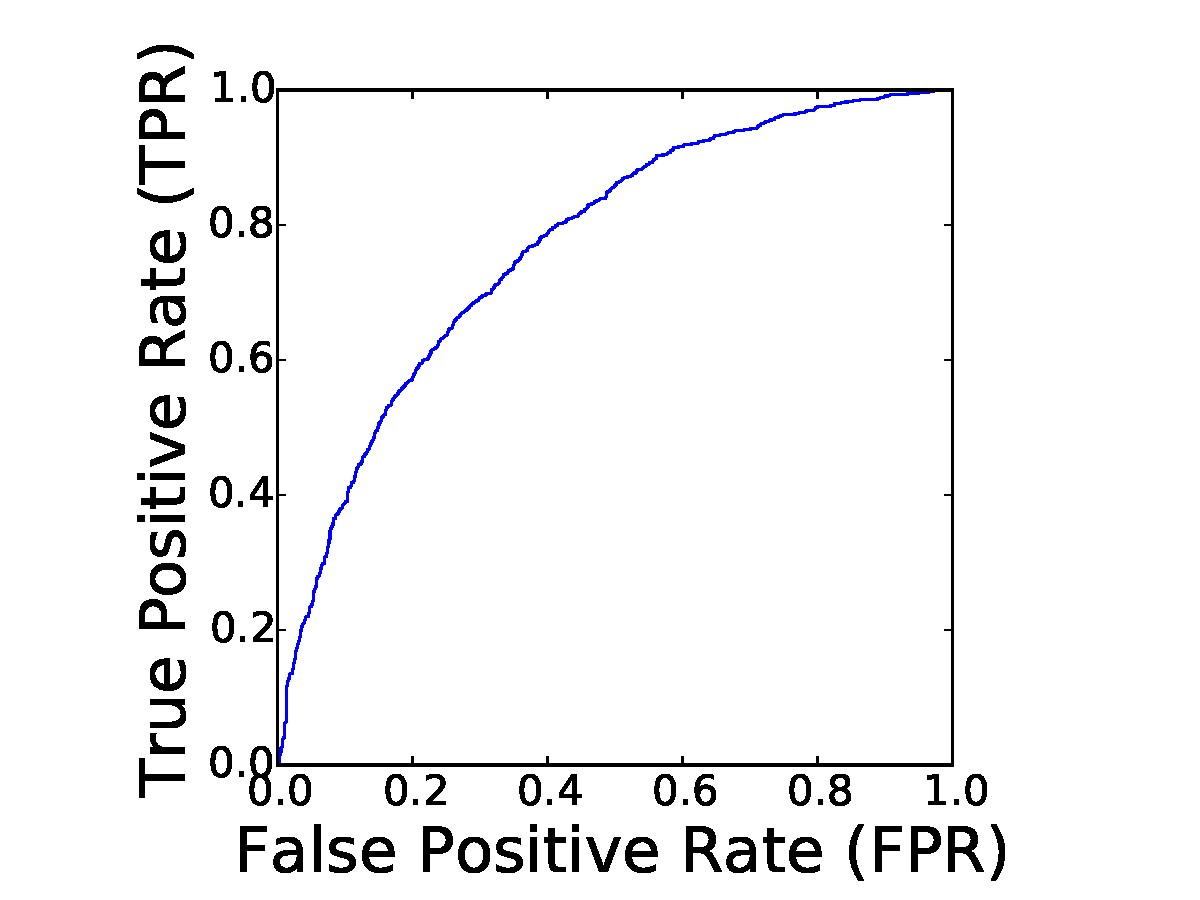
\includegraphics[width=\textwidth]{pic/ROC_sfp.pdf}
\caption{prediction of Sfp labeling activity}
\end{subfigure}
\begin{subfigure}[b]{0.3\linewidth}
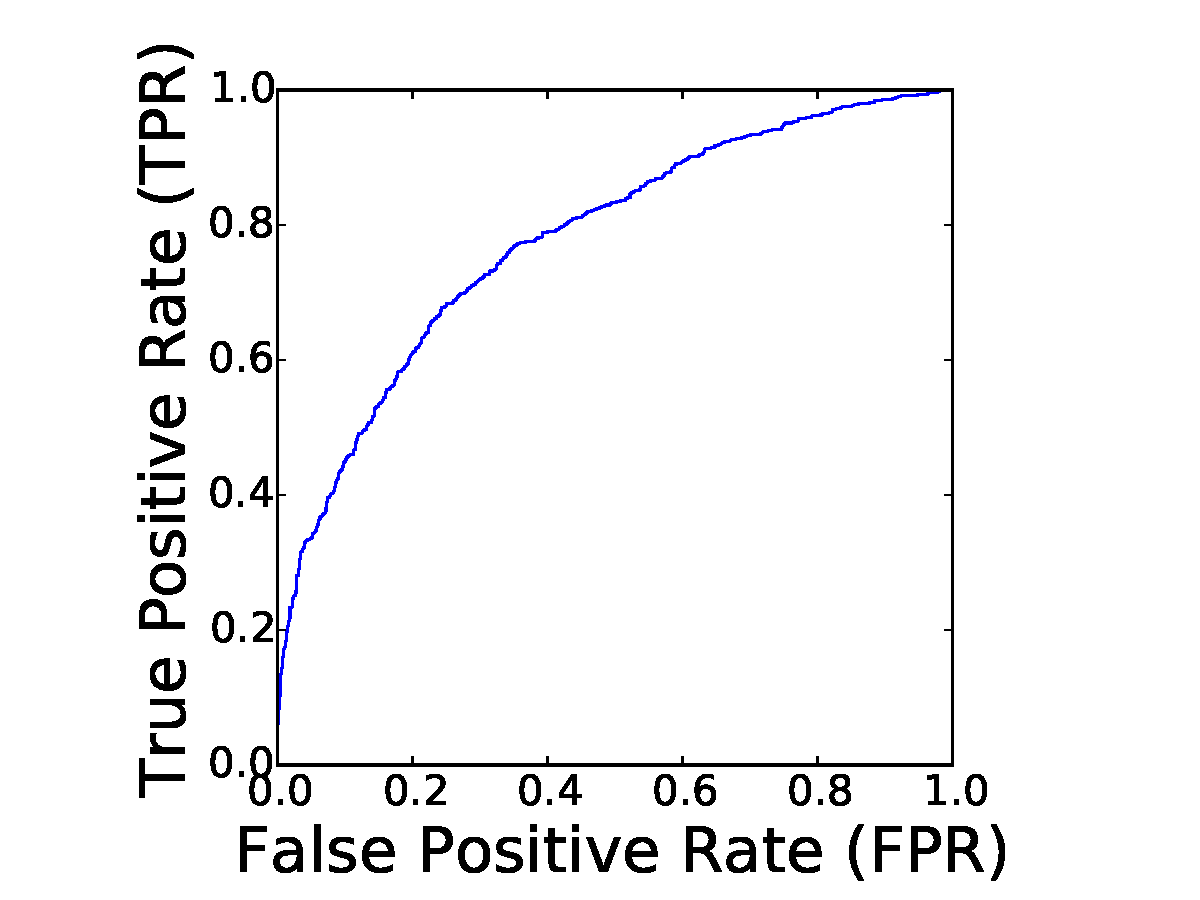
\includegraphics[width=\textwidth]{pic/ROC_AcpS.pdf}
\caption{prediction of AcpS labeling activity}
\end{subfigure}
\begin{subfigure}[b]{0.3\linewidth}
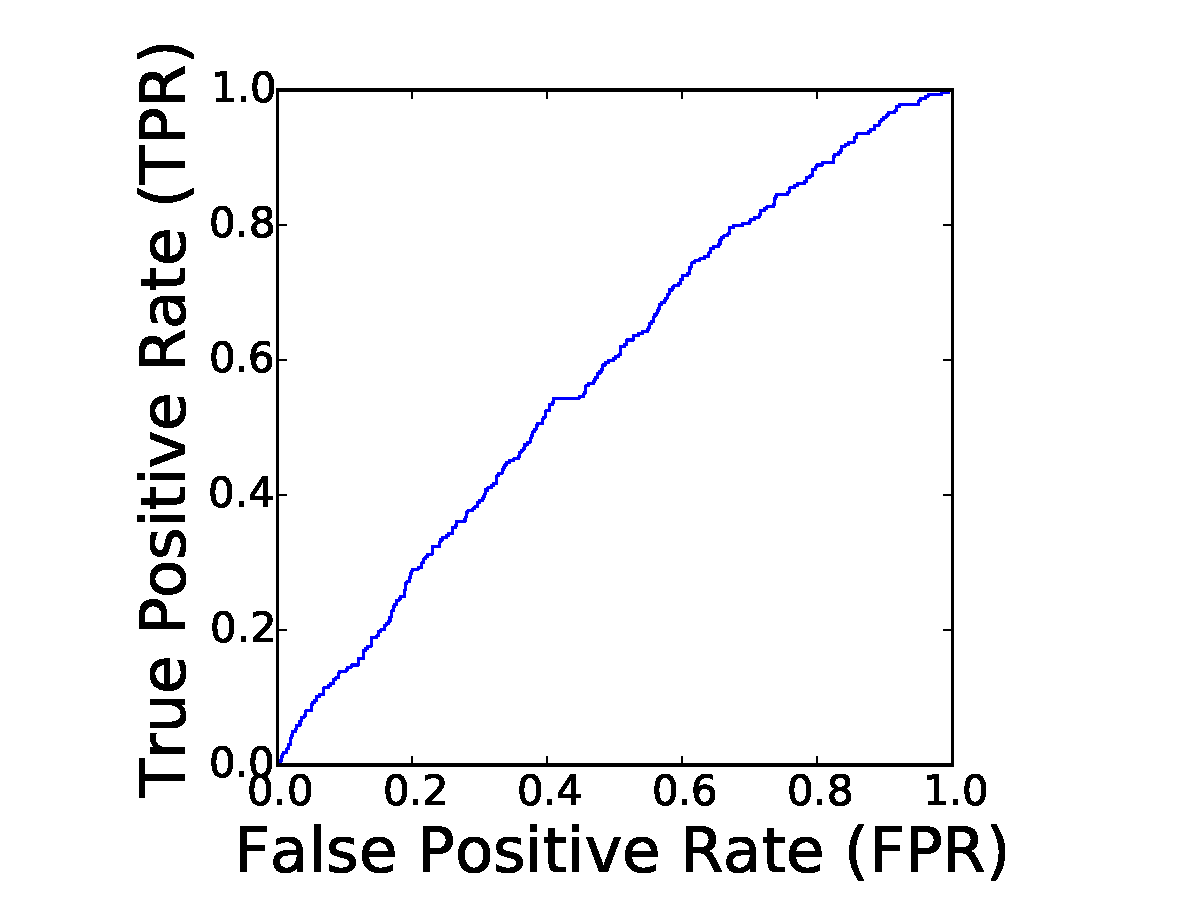
\includegraphics[width=\textwidth]{pic/ROC_PfAcpH.pdf}
\caption{prediction of ACPH unlabeling activity}
\end{subfigure}
\caption{ ROC curve generated by cross validation on all peptides tested so far, which contains Sfp activity for 2602 peptides, AcpS activity for 2022 peptides and ACPH activity for 1380 peptides.}
\label{fig:ROC}
\end{figure}

The classifier performs well if the ROC curve points toward upper left corner, and has no prediction power if the curve is a straight line between $(0,0)$ and $(1,1)$. From the plots we can see the models predicting Sfp and AcpS activity perform very well, but the model predicting ACPH activity has less indicating power.


\subsubsection{Comparison of POOL vs. existing methods}
To illustrate performance of our approach versus existing methods, we simulate a scenario which is very close to our real application, and compare the quality of recommended peptides generated by each method. To simulate a scenario, we used result of all tested peptides to train the model, like we did in \ref{sec:application_roc}, and treat it as \enquote{oracle}, i.e., whether a peptide is a hit or not is completely determined by this trained model. Then we only reveal part of the data to the competing methods, let them generate recommended peptides, and use \enquote{oracle} to evaluate quality of the recommendations produced by the methods. In this experiment, we revealed test result from the first two rounds of experiments, which contain Sfp activity for 847 peptides, AcpS activity for 267 peptides and ACPH activity for 452 peptides. There are only four \enquote{Sfp-specific hits} and one \enquote{AcpS-specific hit} in this revealed dataset. We compare the performance of three methods: they are POOL, which is our proposed approach; predict-then-optimize, discussed in \ref{sec:existing approaches}; mutation method, which is to generate new peptides by mutating existing hits. Each method generates 100 peptides, and we evaluate the quality by calculating the probability of at least one of the recommended peptides is a hit according to \enquote{oracle}. The benchmark plot is shown in Figure~\ref{fig:benchmark}.
\begin{figure}[hpt] 
\center
\begin{subfigure}[b]{0.46\linewidth}
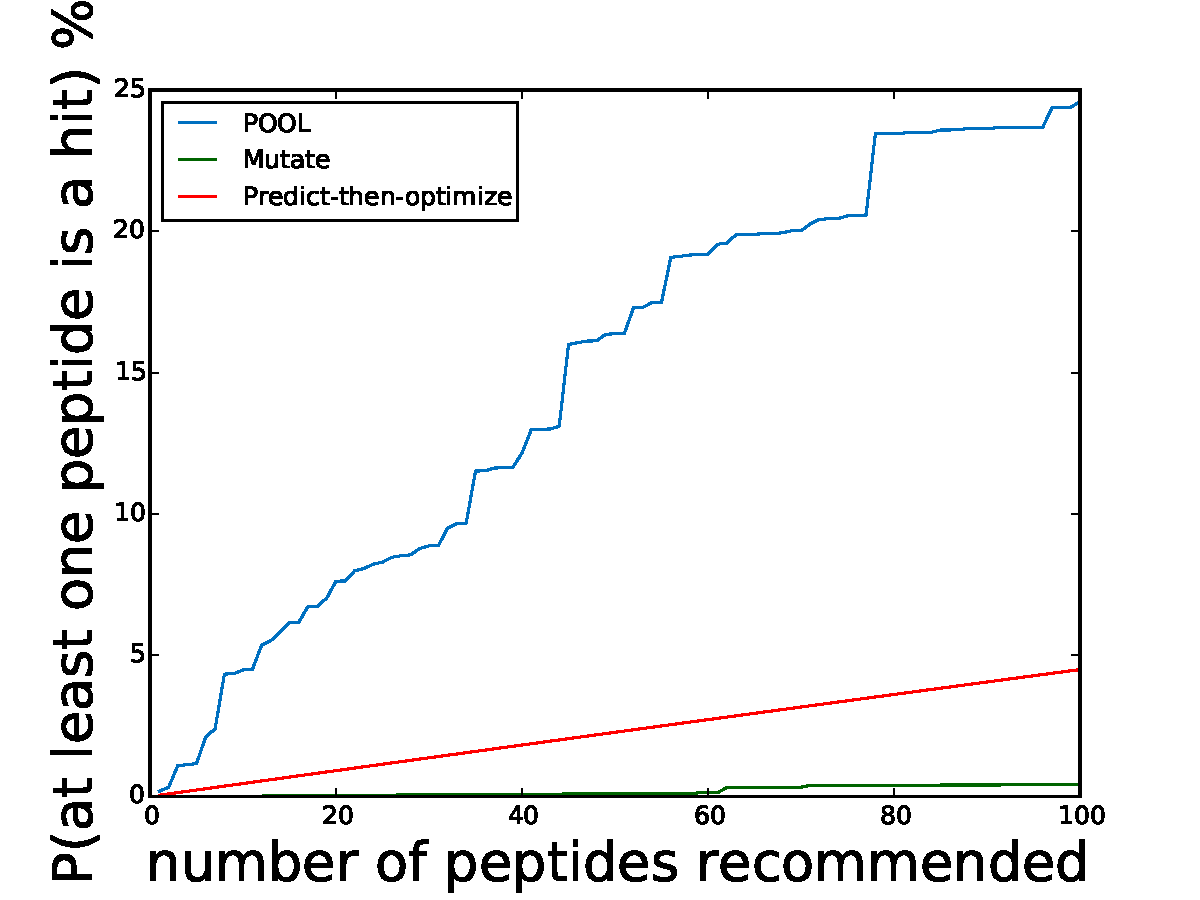
\includegraphics[width=\textwidth]{pic/benchmark_type1.pdf}
\caption{\enquote{Sfp-specific hit}}
\end{subfigure}
\begin{subfigure}[b]{0.46\linewidth}
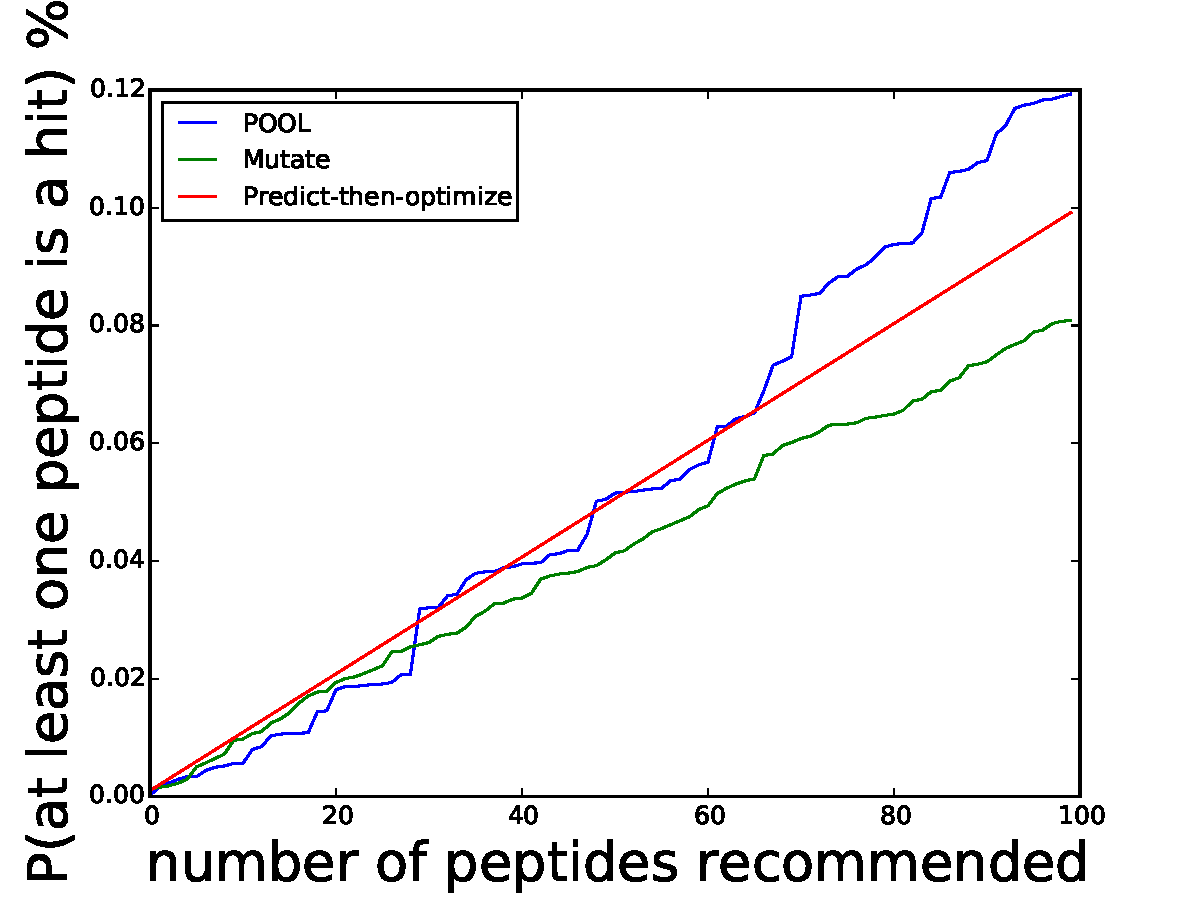
\includegraphics[width=\textwidth]{pic/benchmark_type2.pdf}
\caption{\enquote{AcpS-specific hit}}
\end{subfigure}
\caption{Comparison of quality of recommended peptides by POOL, mutation method and predict-then-optimize approach.}
\label{fig:benchmark}
\end{figure}

From the benchmark we can see POOL beats the other two methods by a significant margin in searching \enquote{Sfp-specific hits}. In the search of \enquote{AcpS-specific hits}, all three methods have similar performance, with POOL achieving a little better, but the recommended peptides have a very low probability that at least one of them is actually a hit according to \enquote{oracle}. This is because the methods only observed one \enquote{AcpS-specific hit}, and it is too hard for the methods to provide high quality peptides given this little information. 

\section{General materials and methods}
\section{Lead peptides with fluorophores}
\section{Sequence alignment of lead peptides}
\part{Supplementary Figures}
\part{Supplementary Tables}
  \begin{center}
\begin{tabular}{| l | c | c | c | c | c | c | c | r|}
\hline
\text{class} & 1 & 2 & 3 & 4 & 5 & 6 & 7 & 8 \\
\hline
\text{Amino Acid} & \text{DE} & \text{NQ} & \text{FWY} &\text{RHK} & \text{AILMV} &\text{GP} &\text{ST} &\text{C} \\
\hline
\end{tabular}
\captionof{table}{Reduced Amino Acid Class} \label{table:reduced aa}
\end{center}

\bibliography{SI}
\bibliographystyle{abbrv}
%%%%%%%%%%%%%%%%%
\end{document}
%%%%%%%%%%%%%%%%%
